\documentclass{article}

% --- OVERLEAF COMPATIBLE PREAMBLE ---
\usepackage[margin=1in]{geometry}
\usepackage[utf8]{inputenc}
\usepackage[T1]{fontenc}
\usepackage[english]{babel}
\usepackage{graphicx}

% Set font to Sans Serif (Helvetica) to approximate Calibri
\usepackage{helvet}
\renewcommand{\familydefault}{\sfdefault}

% --- USER SPECIFIC PACKAGES ---
\usepackage{amsmath}
\usepackage{booktabs}
\usepackage{xcolor}
\usepackage{colortbl}
\usepackage{float}
\usepackage{subcaption}
\usepackage{parskip} % paragraph spacing
\setlength{\parskip}{1em}

% Reduce spacing around and between floats (tables)
\setlength{\floatsep}{4pt}
\setlength{\textfloatsep}{8pt}
\setlength{\intextsep}{4pt}

\setcounter{secnumdepth}{0}

% Define custom colors to match the image data
\definecolor{trueyellow}{HTML}{FFFF00}
\definecolor{meangreen}{HTML}{90EE90}
\definecolor{sigmablue}{HTML}{00CED1}
\definecolor{offpurple}{HTML}{DA70D6}

% Legend colors for Misclassification
\definecolor{negchange}{HTML}{808080} % Gray
\definecolor{improved}{HTML}{558B2F} % Dark Green
\definecolor{greatimproved}{HTML}{A5FF7F} % Bright Green
\definecolor{worsened}{HTML}{FF8A8A} % Light Red
\definecolor{greatworsened}{HTML}{8B0000} % Dark Red



% --- DOCUMENT METADATA ---
\title{Programming Assignment 2 \\ \large Maximum Likelihood Estimation \\ CS 479}
\author{Jackson Loughmiller}
\date{April 7, 2026}

\begin{document}

% Title and Declaration Page
\begin{titlepage}
    \centering
    \vspace*{\fill}
    
    {\huge \textbf{Programming Assignment 2}} \\
    \vspace{0.5cm}
    {\Large Maximum Likelihood Estimation} \\
    \vspace{0.5cm}
    {\large CS 479}
    
    \vspace{2cm}
    
    {\large Jackson Loughmiller} \\
    \vspace{0.2cm}
    {\large April 7, 2026}
    
    \vspace{3cm}
    
    \noindent I declare that all material in this assignment is my own work except
    where there is clear acknowledgment or reference to the work of others.
    I understand that both my report and code may be subjected to plagiarism
    detection software, and fully accept all consequences if found
    responsible for plagiarism, as explained in the syllabus, and described
    in UNR's Academic Standards Policy: UAM 6,502.
    
    \vspace*{\fill}
\end{titlepage}

\newpage

\section{Theory}\label{theory}

\subsection{Experiment 1 \& 2}\label{experiment-1}

\subsubsection*{Parameter Estimation}\label{parameter-estimation}

When using Bayesian classifiers in the practice, it generally cannot be
assumed that one knows the exact parameters of the distribution of their
data. Therefore there must be some technique to estimate those
parameters based on the available training data, that has been
pre-annotated by humans. The parameters that need to be estimated are
the parameters of the likelihood function, shown below in Eq. 1.1:

\begin{equation}
p(x|w_{i}) \sim N(\mu, \Sigma), \quad x \in R^{N}
\label{eq:1.1}
\end{equation}

$p(x|w_{i})$ can also be denoted as $p(x|\theta)$, where
$\theta = (\mu, \Sigma)$ are the parameters of the distribution. The
overall goal of parameter estimation is to determine the best $\theta$
given our data, $D$.

\subsubsection*{Maximum Likelihood Estimation}\label{maximum-likelihood-estimation}

Maximum likelihood estimation is one method of parameter estimation,
that makes a point estimate, $\widehat{\theta}$, by maximizing the
likelihood of obtaining the samples observed in the training data, $D$,
from the distribution $p(x|\widehat{\theta})$. It assumes the
parameters $\theta$ are fixed, unknown quantities. The equation for
$\widehat{\theta}$ is shown below in Eq. 1.2:

\begin{equation}
\widehat{\theta} = \arg\max_{\theta} p(D|\theta)
\label{eq:1.2}
\end{equation}

Assuming all the samples $x_{1}, x_{2}, \dots, x_{n}$ are drawn
independently from $p(x|\theta)$, $p(D|\theta)$ is given by Eq. 1.3,
below:

\begin{equation}
p(D|\theta) = \prod_{k=1}^{n} p(x_{k}|\theta)
\label{eq:1.3}
\end{equation}

\begin{equation}
\ln p(D|\theta) = \sum_{k=1}^{n} \ln(p(x_{k}|\theta))
\label{eq:1.4}
\end{equation}

Now, maximizing $\ln p(D|\theta)$ is equivalent to maximizing
$p(D|\theta)$. This maximum can be found by finding the point where
the gradient of $\ln p(D|\theta)$ is equal to zero, shown below in Eq. 1.5:

\begin{equation}
\nabla_{\theta}\ln p(D|\theta) = 0
\label{eq:1.5}
\end{equation}

The parameters of $\theta$, $\widehat{\mu}$ (sample mean) and
$\widehat{\Sigma}$ (sample covariance) are given by Eqs. 1.6 and 1.7,
respectively:

\begin{equation}
\widehat{\mu} = \frac{1}{n}\sum_{k=1}^{n}x_{k}
\label{eq:1.6}
\end{equation}

\begin{equation}
\widehat{\Sigma} = \frac{1}{n}\sum_{k=1}^{n}(x_{k} - \widehat{\mu})(x_{k} - \widehat{\mu})^{t}
\label{eq:1.7}
\end{equation}

\subsection{Experiment 3}\label{experiment-3}
\subsubsection{Error Rates}\label{Error Rates}
Two widely used error rates are the False Positive Rate (FPR) and the False Negative Rate (FNR). These rates are defined in Eq. 8,
below:

\begin{equation}
\text{FPR} = \frac{FP}{FP + TN}, \qquad \text{FNR} = \frac{FN}{FN + TP}
\label{eq:1.8}
\end{equation}

Where FP is the total count of False Positives, TN is the total count of True Negatives, FN is the total count of False 
Negatives, and TP is the total count of True Positives. These rates can be used to help quantify the performance 
of a given classifier. These rates can be plotted against each other on the same graph, with Error Rate as the y-axis 
and a theshold value, t, as the x-axis. The value of t at which the lines intersect on this graph is known as the 
Equal Error Rate (EER), which is commonly used to choose a value for the parameter t. 

\subsubsection{ROC Curves}\label{ROC Curves}
Receiver Operator Characteristic (ROC) Curves are a method to compare different thresholds for a single classifier. They can also
be used to compare multiple classifiers that are attempting to classify the same states of nature. The most commonly used ROC curve is 
obtained by plotting the FPR against the FNR, and the classifier that minimizes the area under this curve would would be considered
the better performing classifier. 

\subsubsection{Color Spaces}\label{Color Spaces}
The standard encoding used in most color images is RGB, which is a method that stores 3 values for each pixel in an image. 
The three values encode the red, green, and blue parts of the pixels color. This method works well for encoding images
and displaying them for humans, but is not the most ideal for classifying skin color in an image. Instead, one can convert
RGB values to a different chromatic space. The normalized RGB space, shown below in Eq. 9, removes the luminance component 
from the representation by dividing by the total intensity of the pixel value:

\begin{equation}
r = \frac{R}{R + G + B}, \qquad g = \frac{G}{R + G + B}
\label{eq:chromatic1}
\end{equation}

The YCbCr color space, on the other hand, does not discard the luminance component, but instead separates it. For skin classification
purpose, the Y component can be discarded to classify based only on color information. The method for converting to this space 
is shown below in Eq. 10:

\begin{equation}
\begin{aligned}
Y  &= 0.299R + 0.587G + 0.114B \\
C_b &= -0.169R - 0.332G + 0.500B \\
C_r &= 0.500R - 0.419G - 0.081B
\end{aligned}
\label{eq:chromatic2}
\end{equation}

\section{Results and Discussion}\label{results-and-discussion}

\subsection{Experiment 1}\label{experiment-1-1}
\noindent For this experiment, data was generated in the same manner as the first assignment, using the following parameters for the multivariate 
Guassian distribution: 

\begin{equation}
\mu_{1} = \begin{bmatrix} 1 \\ 1 \end{bmatrix}, 
\quad \Sigma_{1} = \begin{bmatrix} 1 & 0 \\ 0 & 1 \end{bmatrix}, 
\quad \mu_{2} = \begin{bmatrix} 4 \\ 4 \end{bmatrix}, 
\quad \Sigma_{2} = \begin{bmatrix} 1 & 0 \\ 0 & 1 \end{bmatrix}
\label{eq:exp1_params}
\end{equation}

\noindent A total of 200,000 samples were generated, 60,000 from $\mu_{1}$ and $\Sigma_{1}$, and 140,000 from $\mu_{2}$ and $\Sigma_{2}$. Parameters were 
then estimated using Maximum Likelihood Estimation on 100\%, 10\%, 1\%, 0.1\%, and 0.01\% of the data set. Tables 1 and 2, below, 
show the real and estimated parameters for different sample sizes of the dataset. As the tables show, the parameters get 
progressively farther away from the true parameters as the sample size decreases. 

\begin{table}[H]
\centering
\small
\caption{Class 1 - Estimated Parameters vs. True Parameters}
\vspace{-0.4em}
\begin{tabular}{ccccccc}
\toprule
\textbf{Sample} & \textbf{mu1\_x} & \textbf{mu1\_y} & \textbf{sigma1\_11} & \textbf{sigma1\_12} & \textbf{sigma1\_21} & \textbf{sigma1\_22} \\
\midrule
\textbf{True} & \cellcolor{trueyellow} 1.0000 & \cellcolor{trueyellow} 1.0000 & \cellcolor{trueyellow} 1.0000 & \cellcolor{trueyellow} 0.0000 & \cellcolor{trueyellow} 0.0000 & \cellcolor{trueyellow} 1.0000 \\
\textbf{100\%} & \cellcolor{meangreen} 1.0049 & \cellcolor{meangreen} 0.9960 & \cellcolor{sigmablue} 1.0037 & \cellcolor{offpurple} 0.0014 & \cellcolor{offpurple} 0.0014 & \cellcolor{sigmablue} 1.0034 \\
\textbf{10\%} & \cellcolor{meangreen} 1.0158 & \cellcolor{meangreen} 0.9724 & \cellcolor{sigmablue} 0.9784 & \cellcolor{offpurple} -0.0201 & \cellcolor{offpurple} -0.0201 & \cellcolor{sigmablue} 1.0050 \\
\textbf{1\%} & \cellcolor{meangreen} 1.0130 & \cellcolor{meangreen} 0.9815 & \cellcolor{sigmablue} 0.9317 & \cellcolor{offpurple} 0.0019 & \cellcolor{offpurple} 0.0019 & \cellcolor{sigmablue} 1.0601 \\
\textbf{0.1\%} & \cellcolor{meangreen} 1.0228 & \cellcolor{meangreen} 1.1984 & \cellcolor{sigmablue} 1.0328 & \cellcolor{offpurple} -0.0435 & \cellcolor{offpurple} -0.0435 & \cellcolor{sigmablue} 1.1159 \\
\textbf{0.01\%} & \cellcolor{meangreen} 0.7019 & \cellcolor{meangreen} 1.4115 & \cellcolor{sigmablue} 0.7182 & \cellcolor{offpurple} -0.1377 & \cellcolor{offpurple} -0.1377 & \cellcolor{sigmablue} 0.5233 \\
\bottomrule
\end{tabular}
\end{table}

\begin{table}[H]
\centering
\small
\caption{Class 2 - Estimated Parameters vs. True Parameters}
\vspace{-0.4em}
\begin{tabular}{ccccccc}
\toprule
\textbf{Sample} & \textbf{mu2\_x} & \textbf{mu2\_y} & \textbf{sigma2\_11} & \textbf{sigma2\_12} & \textbf{sigma2\_21} & \textbf{sigma2\_22} \\
\midrule
\textbf{True} & \cellcolor{trueyellow} 4.0000 & \cellcolor{trueyellow} 4.0000 & \cellcolor{trueyellow} 1.0000 & \cellcolor{trueyellow} 0.0000 & \cellcolor{trueyellow} 0.0000 & \cellcolor{trueyellow} 1.0000 \\
\textbf{100\%} & \cellcolor{meangreen} 3.9997 & \cellcolor{meangreen} 4.0044 & \cellcolor{sigmablue} 1.0015 & \cellcolor{offpurple} -0.0005 & \cellcolor{offpurple} -0.0005 & \cellcolor{sigmablue} 1.0015 \\
\textbf{10\%} & \cellcolor{meangreen} 3.9955 & \cellcolor{meangreen} 4.0133 & \cellcolor{sigmablue} 1.0105 & \cellcolor{offpurple} 0.0087 & \cellcolor{offpurple} 0.0087 & \cellcolor{sigmablue} 1.0154 \\
\textbf{1\%} & \cellcolor{meangreen} 3.9794 & \cellcolor{meangreen} 4.0238 & \cellcolor{sigmablue} 1.0229 & \cellcolor{offpurple} 0.0042 & \cellcolor{offpurple} 0.0042 & \cellcolor{sigmablue} 0.9445 \\
\textbf{0.1\%} & \cellcolor{meangreen} 4.1308 & \cellcolor{meangreen} 3.9784 & \cellcolor{sigmablue} 0.9435 & \cellcolor{offpurple} -0.0139 & \cellcolor{offpurple} -0.0139 & \cellcolor{sigmablue} 0.8722 \\
\textbf{0.01\%} & \cellcolor{meangreen} 4.0347 & \cellcolor{meangreen} 4.0391 & \cellcolor{sigmablue} 1.1736 & \cellcolor{offpurple} 0.3776 & \cellcolor{offpurple} 0.3776 & \cellcolor{sigmablue} 1.1840 \\
\bottomrule
\end{tabular}
\end{table}

\begin{center}
\textbf{Parameter Legend} \\
\begin{tabular}{|l|l|}
\hline
\cellcolor{trueyellow} & True reference values \\ \hline
\cellcolor{meangreen} & Mean (mu) \\ \hline
\cellcolor{sigmablue} & Diagonal sigma (11, 22) \\ \hline
\cellcolor{offpurple} & Off-diagonal sigma (12, 21) \\ \hline
\end{tabular}
\end{center}

\noindent The estimated parameters stay within 1 decimal of accuracy, until the dataset was reduced to 0.1\% of its original size. This indicates
that the methods used do not require a massive amount of data to be relatively accurate, and this will be shown in more detail in the 
misclassification rates.  

\noindent Tables 3-5, below, show the misclassification rates for each sample size. As shown by the tables, there is only negligible difference in the rates until the 
sample size reaches 0.1\% of the original dataset size. The difference is most significant in the set that contains only 0.01\% 
of the original training data, with a 42.83\% increase in the total misclassification rate, going from 1.5620\% for 
the real parameters, to 2.2310\% for the estimated parameters. 

\begin{table}[H]
\centering
\small
\caption{W1 Misclassification Rates}
\vspace{-0.4em}
\begin{tabular}{cccc}
\toprule
\textbf{Sample Size} & \textbf{Real Params} & \textbf{Estimated Params} & \textbf{Zeroed Diag} \\
\midrule
\textbf{0.01\%} & 2.7883\% & 6.6500\% & 4.7517\% \\
\textbf{0.1\%} & 2.7883\% & 1.8400\% & 1.8150\% \\
\textbf{1\%} & 2.7883\% & 2.7483\% & 2.7400\% \\
\textbf{10\%} & 2.7883\% & 2.9417\% & 2.8617\% \\
\textbf{100\%} & 2.7883\% & 2.7683\% & 2.7767\% \\
\bottomrule
\end{tabular}
\end{table}

\begin{table}[H]
\centering
\small
\caption{W2 Misclassification Rates}
\vspace{-0.4em}
\begin{tabular}{cccc}
\toprule
\textbf{Sample Size} & \textbf{Real Params} & \textbf{Estimated Params} & \textbf{Zeroed Diag} \\
\midrule
\textbf{0.01\%} & 1.0364\% & 0.3371\% & 0.6093\% \\
\textbf{0.1\%} & 1.0364\% & 1.6236\% & 1.6400\% \\
\textbf{1\%} & 1.0364\% & 1.0486\% & 1.0536\% \\
\textbf{10\%} & 1.0364\% & 0.9814\% & 1.0071\% \\
\textbf{100\%} & 1.0364\% & 1.0429\% & 1.0407\% \\
\bottomrule
\end{tabular}
\end{table}

\begin{table}[H]
\centering
\small
\caption{Total Misclassification Rates}
\vspace{-0.4em}
\begin{tabular}{cccc}
\toprule
\textbf{Sample Size} & \textbf{Real Params} & \textbf{Estimated Params} & \textbf{Zeroed Diag} \\
\midrule
\textbf{0.01\%} & 1.5620\% & 2.2310\% & 1.8520\% \\
\textbf{0.1\%} & 1.5620\% & 1.6885\% & 1.6925\% \\
\textbf{1\%} & 1.5620\% & 1.5585\% & 1.5595\% \\
\textbf{10\%} & 1.5620\% & 1.5695\% & 1.5635\% \\
\textbf{100\%} & 1.5620\% & 1.5605\% & 1.5615\% \\
\bottomrule
\end{tabular}
\end{table}

The tables show a marginal decrease in the misclassification rate for the 0.01\% sample size when the non-diagonal values of the estimated covariance matrix are zero'd out, 
reducing the rate from 2.23\% to 1.85\%. This indicates that with a small number of data, zeroing out the non-diagonal values of the estimated covariance matrix could 
improve performance slightly, however this would likely depend on the actual parameters. 

\subsection{Experiment 2}\label{experiment-2-1}
\noindent For this experiment, the data was generated in the same manner as experiment 1, using the following parameters in Eq. \ref{eq:exp2_params}: 

\begin{equation}
\mu_{1} = \begin{bmatrix} 1 \\ 1 \end{bmatrix}, 
\quad \Sigma_{1} = \begin{bmatrix} 1 & 0 \\ 0 & 1 \end{bmatrix}, 
\quad \mu_{2} = \begin{bmatrix} 4 \\ 4 \end{bmatrix}, 
\quad \Sigma_{2} = \begin{bmatrix} 4 & 0 \\ 0 & 8 \end{bmatrix}
\label{eq:exp2_params}
\end{equation}

\noindent As seen by tables 6-7, below, the results follow a similar pattern to experiment 1, with the parameter values straying further from the true values
as the sample size decreases. 

\begin{table}[H]
\centering
\small
\caption{Class 1 - Estimated Parameters vs. True Parameters}
\vspace{-0.4em}
\begin{tabular}{ccccccc}
\toprule
\textbf{Sample} & \textbf{mu1\_x} & \textbf{mu1\_y} & \textbf{sigma1\_11} & \textbf{sigma1\_12} & \textbf{sigma1\_21} & \textbf{sigma1\_22} \\
\midrule
\textbf{True} & \cellcolor{trueyellow} 1.0000 & \cellcolor{trueyellow} 1.0000 & \cellcolor{trueyellow} 1.0000 & \cellcolor{trueyellow} 0.0000 & \cellcolor{trueyellow} 0.0000 & \cellcolor{trueyellow} 1.0000 \\
\textbf{100\%} & \cellcolor{meangreen} 1.0049 & \cellcolor{meangreen} 0.9960 & \cellcolor{sigmablue} 1.0037 & \cellcolor{offpurple} 0.0014 & \cellcolor{offpurple} 0.0014 & \cellcolor{sigmablue} 1.0034 \\
\textbf{10\%} & \cellcolor{meangreen} 1.0158 & \cellcolor{meangreen} 0.9724 & \cellcolor{sigmablue} 0.9784 & \cellcolor{offpurple} -0.0201 & \cellcolor{offpurple} -0.0201 & \cellcolor{sigmablue} 1.0050 \\
\textbf{1\%} & \cellcolor{meangreen} 1.0130 & \cellcolor{meangreen} 0.9815 & \cellcolor{sigmablue} 0.9317 & \cellcolor{offpurple} 0.0019 & \cellcolor{offpurple} 0.0019 & \cellcolor{sigmablue} 1.0601 \\
\textbf{0.1\%} & \cellcolor{meangreen} 1.0228 & \cellcolor{meangreen} 1.1984 & \cellcolor{sigmablue} 1.0328 & \cellcolor{offpurple} -0.0435 & \cellcolor{offpurple} -0.0435 & \cellcolor{sigmablue} 1.1159 \\
\textbf{0.01\%} & \cellcolor{meangreen} 0.7019 & \cellcolor{meangreen} 1.4115 & \cellcolor{sigmablue} 0.7182 & \cellcolor{offpurple} -0.1377 & \cellcolor{offpurple} -0.1377 & \cellcolor{sigmablue} 0.5233 \\
\bottomrule
\end{tabular}
\end{table}

\begin{table}[H]
\centering
\small
\caption{Class 2 - Estimated Parameters vs. True Parameters}
\vspace{-0.4em}
\begin{tabular}{ccccccc}
\toprule
\textbf{Sample} & \textbf{mu2\_x} & \textbf{mu2\_y} & \textbf{sigma2\_11} & \textbf{sigma2\_12} & \textbf{sigma2\_21} & \textbf{sigma2\_22} \\
\midrule
\textbf{True} & \cellcolor{trueyellow} 4.0000 & \cellcolor{trueyellow} 4.0000 & \cellcolor{trueyellow} 4.0000 & \cellcolor{trueyellow} 0.0000 & \cellcolor{trueyellow} 0.0000 & \cellcolor{trueyellow} 8.0000 \\
\textbf{100\%} & \cellcolor{meangreen} 3.9994 & \cellcolor{meangreen} 4.0124 & \cellcolor{sigmablue} 4.0061 & \cellcolor{offpurple} -0.0030 & \cellcolor{offpurple} -0.0030 & \cellcolor{sigmablue} 8.0121 \\
\textbf{10\%} & \cellcolor{meangreen} 3.9910 & \cellcolor{meangreen} 4.0376 & \cellcolor{sigmablue} 4.0419 & \cellcolor{offpurple} 0.0493 & \cellcolor{offpurple} 0.0493 & \cellcolor{sigmablue} 8.1234 \\
\textbf{1\%} & \cellcolor{meangreen} 3.9588 & \cellcolor{meangreen} 4.0673 & \cellcolor{sigmablue} 4.0915 & \cellcolor{offpurple} 0.0237 & \cellcolor{offpurple} 0.0237 & \cellcolor{sigmablue} 7.5560 \\
\textbf{0.1\%} & \cellcolor{meangreen} 4.2616 & \cellcolor{meangreen} 3.9390 & \cellcolor{sigmablue} 3.7739 & \cellcolor{offpurple} -0.0785 & \cellcolor{offpurple} -0.0785 & \cellcolor{sigmablue} 6.9775 \\
\textbf{0.01\%} & \cellcolor{meangreen} 4.0695 & \cellcolor{meangreen} 4.1107 & \cellcolor{sigmablue} 4.6942 & \cellcolor{offpurple} 2.1358 & \cellcolor{offpurple} 2.1358 & \cellcolor{sigmablue} 9.4720 \\
\bottomrule
\end{tabular}
\end{table}

\begin{center}
\textbf{Parameter Legend} \\
\begin{tabular}{|l|l|}
\hline
\cellcolor{trueyellow} & True reference values \\ \hline
\cellcolor{meangreen} & Mean (mu) \\ \hline
\cellcolor{sigmablue} & Diagonal sigma (11, 22) \\ \hline
\cellcolor{offpurple} & Off-diagonal sigma (12, 21) \\ \hline
\end{tabular}
\end{center}

\noindent The estimated parameters seem to have a larger margin of error in this experiment as compared to experiment 1. It seems that as the value of the parameters increase 
(sigma2\_22 is 8, while sigma1\_22 is 1), the magnitude of the error increases as well. 

Tables 8-10, below, show the misclassification rates from the previously described dataset. 
\begin{table}[H]
\centering
\small
\caption{W1 Misclassification Rates}
\vspace{-0.4em}
\begin{tabular}{cccc}
\toprule
\textbf{Sample Size} & \textbf{Real Params} & \textbf{Estimated Params} & \textbf{Zeroed Diag} \\
\midrule
\textbf{0.01\%} & 8.6083\% & 23.5667\% & 19.3933\% \\
\textbf{0.1\%} & 8.6083\% & 6.4550\% & 6.5900\% \\
\textbf{1\%} & 8.6083\% & 8.6733\% & 8.6433\% \\
\textbf{10\%} & 8.6083\% & 8.6733\% & 8.6033\% \\
\textbf{100\%} & 8.6083\% & 8.5300\% & 8.5367\% \\
\bottomrule
\end{tabular}
\end{table}

\begin{table}[H]
\centering
\small
\caption{W2 Misclassification Rates}
\vspace{-0.4em}
\begin{tabular}{cccc}
\toprule
\textbf{Sample Size} & \textbf{Real Params} & \textbf{Estimated Params} & \textbf{Zeroed Diag} \\
\midrule
\textbf{0.01\%} & 7.2707\% & 4.7950\% & 5.3771\% \\
\textbf{0.1\%} & 7.2707\% & 8.4414\% & 8.3950\% \\
\textbf{1\%} & 7.2707\% & 7.2814\% & 7.2900\% \\
\textbf{10\%} & 7.2707\% & 7.2500\% & 7.2657\% \\
\textbf{100\%} & 7.2707\% & 7.3057\% & 7.3021\% \\
\bottomrule
\end{tabular}
\end{table}

\begin{table}[H]
\centering
\small
\caption{Total Misclassification Rates}
\vspace{-0.4em}
\begin{tabular}{cccc}
\toprule
\textbf{Sample Size} & \textbf{Real Params} & \textbf{Estimated Params} & \textbf{Zeroed Diag} \\
\midrule
\textbf{0.01\%} & 7.6720\% & 10.4265\% & 9.5820\% \\
\textbf{0.1\%} & 7.6720\% & 7.8455\% & 7.8535\% \\
\textbf{1\%} & 7.6720\% & 7.6990\% & 7.6960\% \\
\textbf{10\%} & 7.6720\% & 7.6770\% & 7.6670\% \\
\textbf{100\%} & 7.6720\% & 7.6730\% & 7.6725\% \\
\bottomrule
\end{tabular}
\end{table}

\noindent In this experiment, there was a more significant increase in the error of the 0.01\% dataset, rising to 10.43\% as compared to the real parameters 
error of 7.67\%, almost a 3\% increase. Zeroing out the non-diagonal values provided a similar performance gain as in experiment 1, taking into account the 
difference in the original error rate, reducing the error by almost 1\%, as opposed to around 0.4\% in experiment 1. 
\subsection{Experiment 3}\label{experiment-3-1}

\noindent In this experiment, I used Maximum Likelihood (ML) estimation to estimate the parameters of the distribution of skin color, 
for the purpose of segmenting out peoples faces in an image. To do this, I applied the same ML estimation function used in experiments 1 and 2
on 1 training image, shown below in Figure 1 (All of the non-black pixels in Figure 1.b are pixels designated as belonging to a persons face). I 
performed this experiment in two parts, a and b. In part a, I trained and tested the classifier in the normalized RGB space (shown in Eq. 9), and 
for part b I trained and tested the classifier in the YCbCr space (shown in Eq. 10). 

\begin{figure}[H]
    \centering
    \begin{subfigure}[t]{0.40\textwidth}
        \centering
        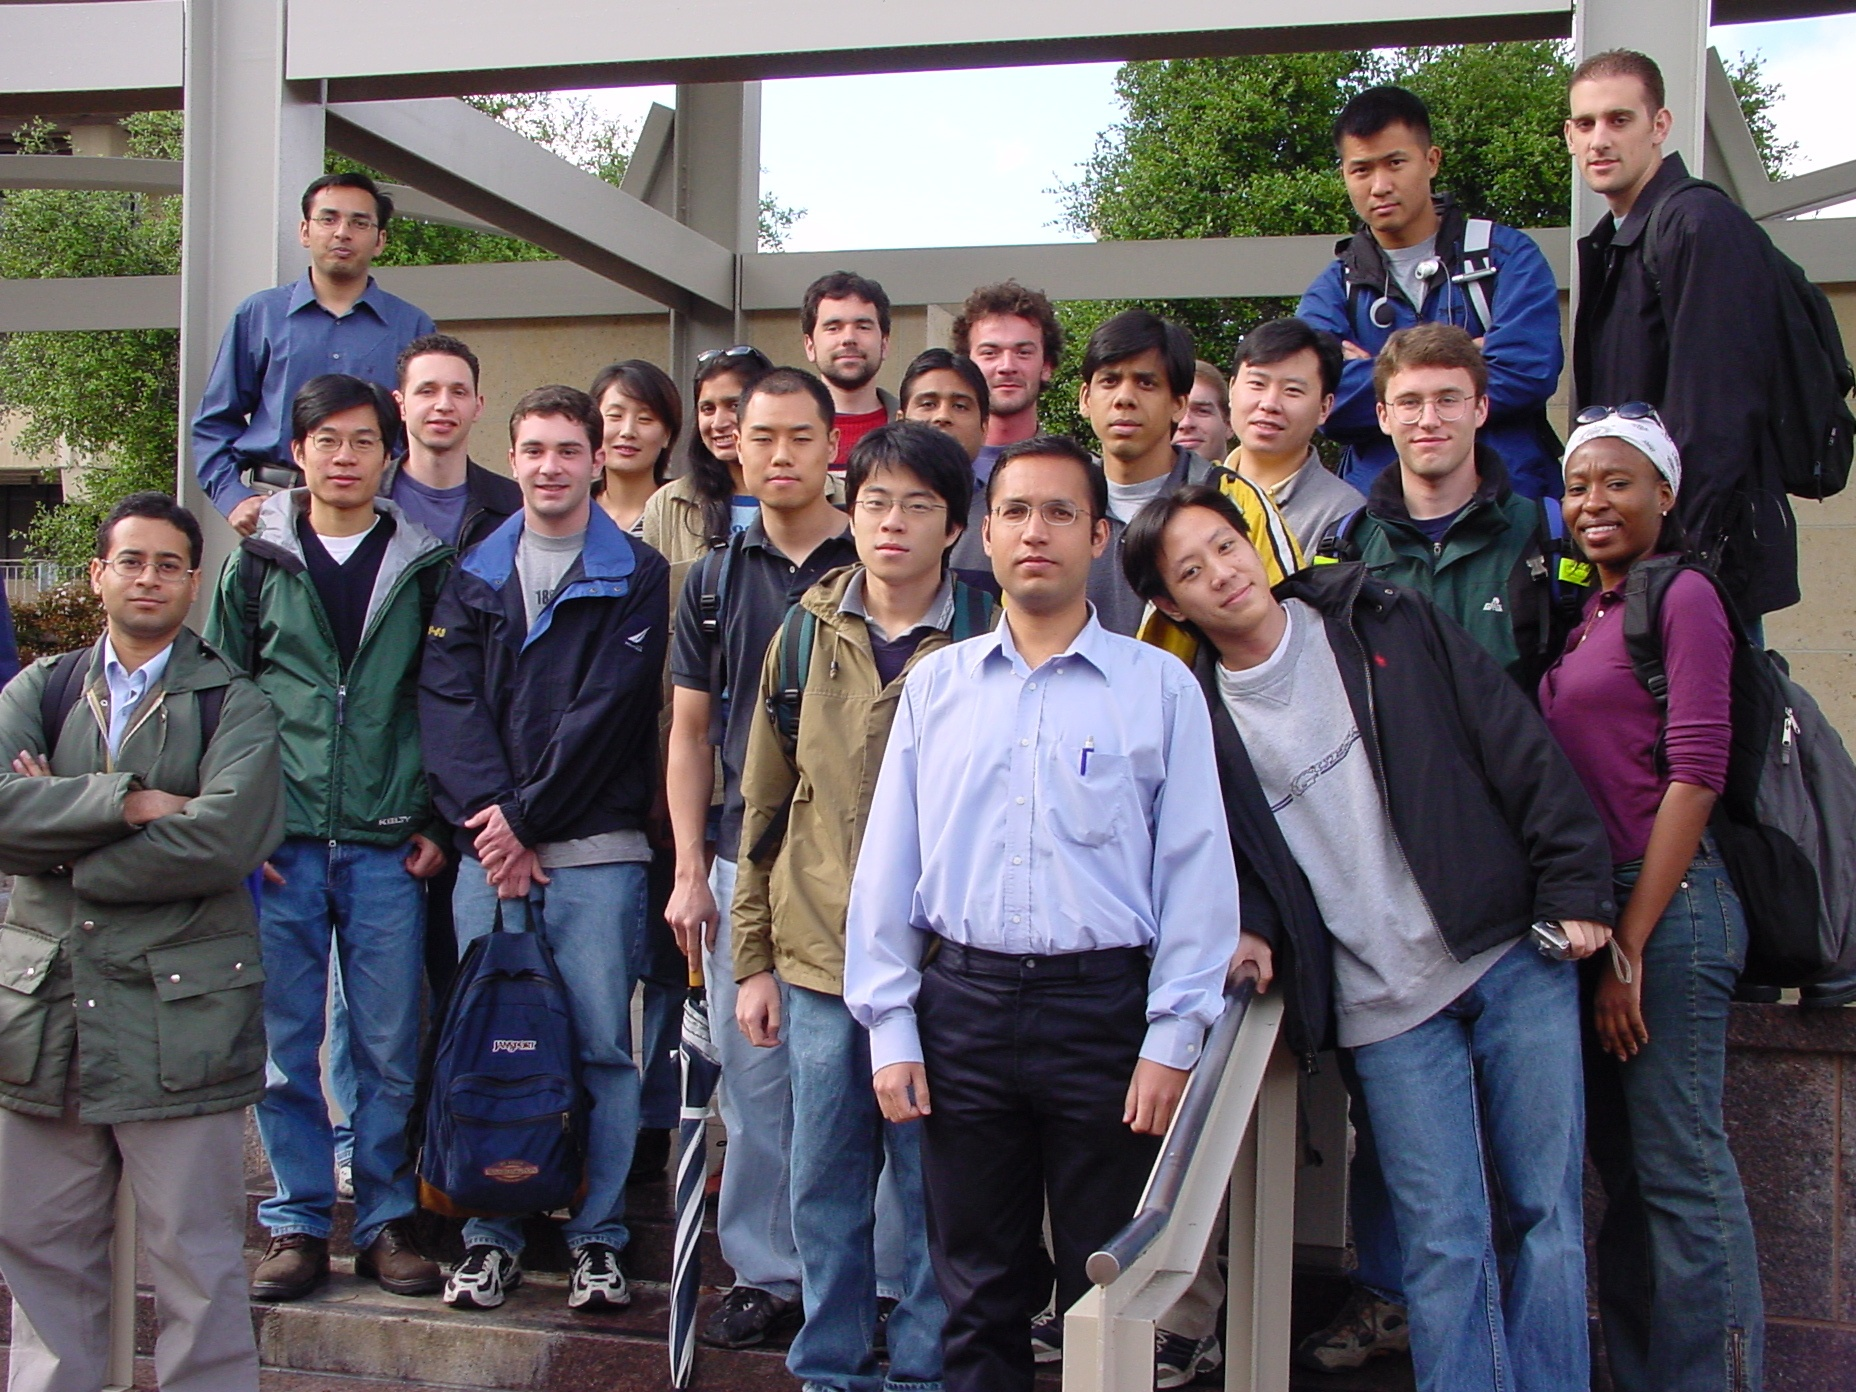
\includegraphics[width=\textwidth]{../output/training_1.jpg}
        \caption{Training image}
    \end{subfigure}
    \begin{subfigure}[t]{0.40\textwidth}
        \centering
        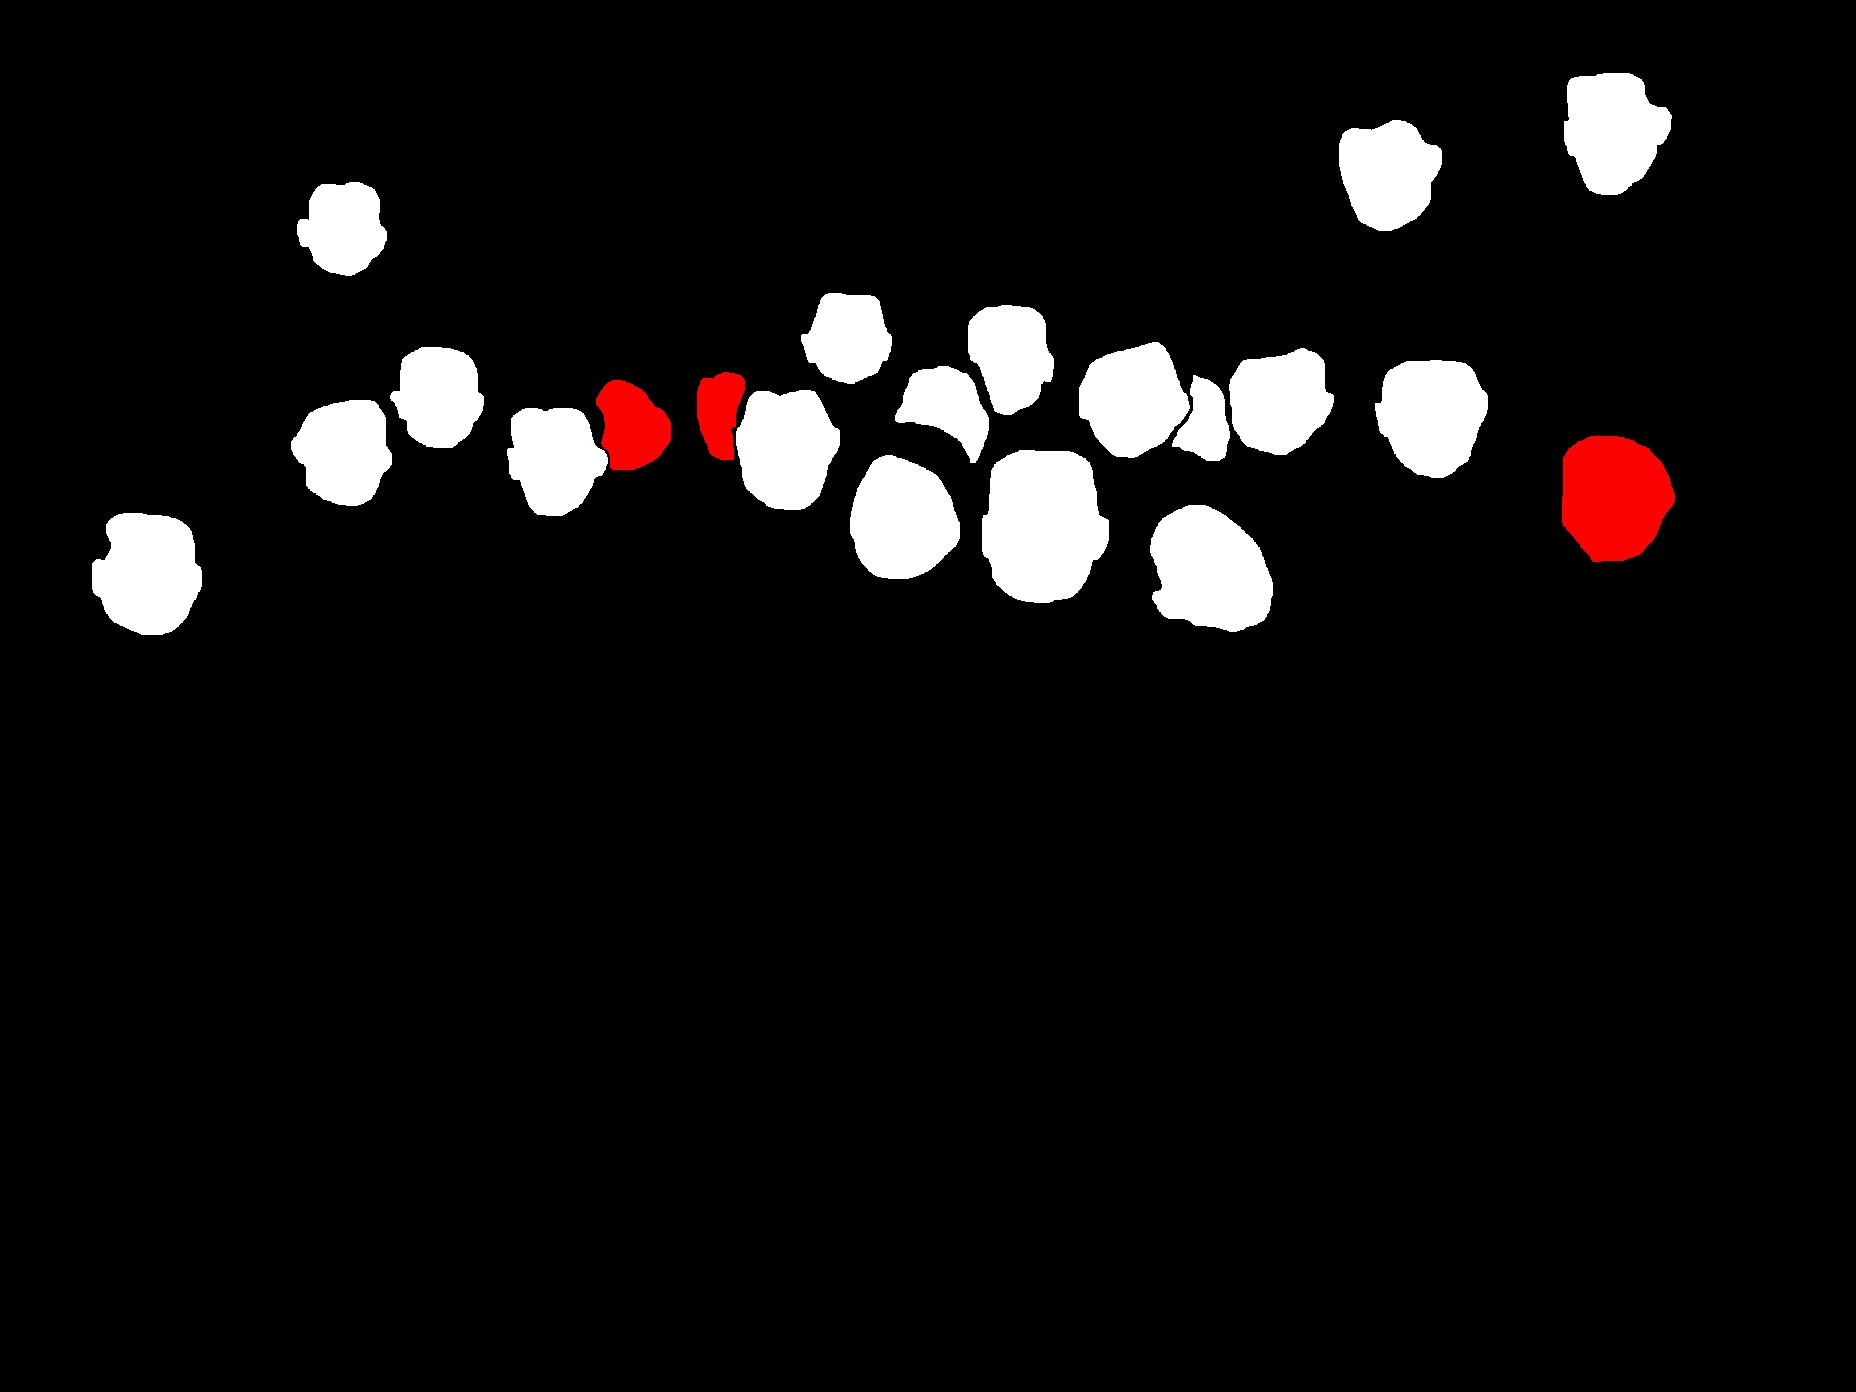
\includegraphics[width=\textwidth]{../output/ref1.jpg}
        \caption{Reference image}
    \end{subfigure}
    \caption{Training and reference image used for estimation}
    \label{fig:training_img}
\end{figure}

To train the classifier, two steps needed to be completed. I needed to estimate the parameters of the distribution (mu and sigma), and 
I needed to estimate the threshold at which the classifier would determine a pixel to be skin or non-skin. To estimate this 
parameter t, I ran the classification function with 10,000 different threshold values (ranging from 0 to c, where $c = \dfrac{1}{2\pi |\Sigma|^{1/2}}$,
and the step size is $\dfrac{c}{10000}$). For each run, I calculated the FPR and FNR, then plotted these rates
on the graphs shown in Figure 2. The intersection of the FPR and FNR on these plots represent the Equal Error Rate (EOR), and the value of t
at these intersections is the threshold I used for classification in the next steps. 

\begin{figure}[H]
    \centering
    \begin{subfigure}[t]{0.48\textwidth}
        \centering
        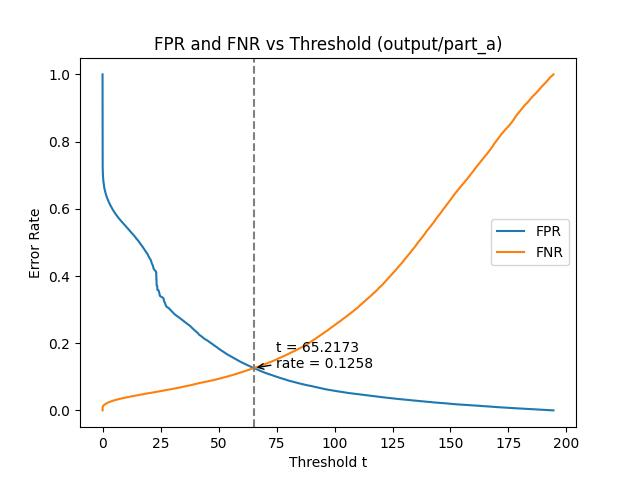
\includegraphics[width=\textwidth]{../output/part_a_roc.jpg}
        \caption{Part A - Normalized RGB ROC Curve}
    \end{subfigure}
    \begin{subfigure}[t]{0.48\textwidth}
        \centering
        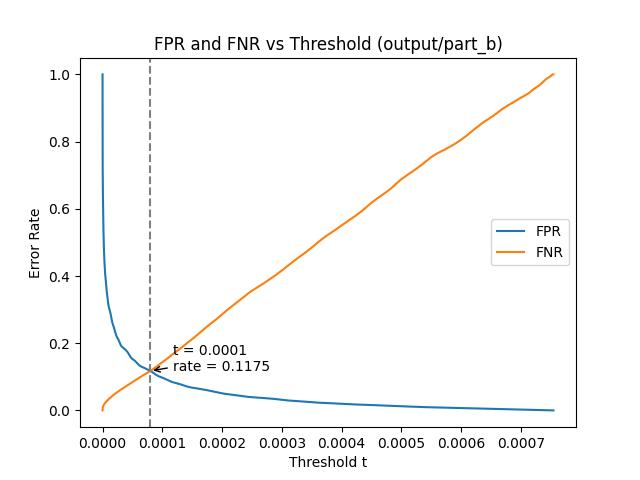
\includegraphics[width=\textwidth]{../output/part_b_roc.jpg}
        \caption{Part B - YCbCr ROC Curve}
    \end{subfigure}
    \caption{ROC Curves for Parts A and B}
    \label{fig:roc-ab}
\end{figure}

Figure 2 shows that the YCbCr space, used in part b, seems to produce less False Positives than part a. 
It did, however, seem to produce more False Negatives. To evaluate the performance of the classifier visually, I used
the t value associated with the EER (given by the intersection of the two plotted lines), and I was able to obtain the 
results shown below in Figures 3 and 4. 

\begin{figure}[H]
    \centering
    \begin{subfigure}[t]{0.35\textwidth}
        \centering
        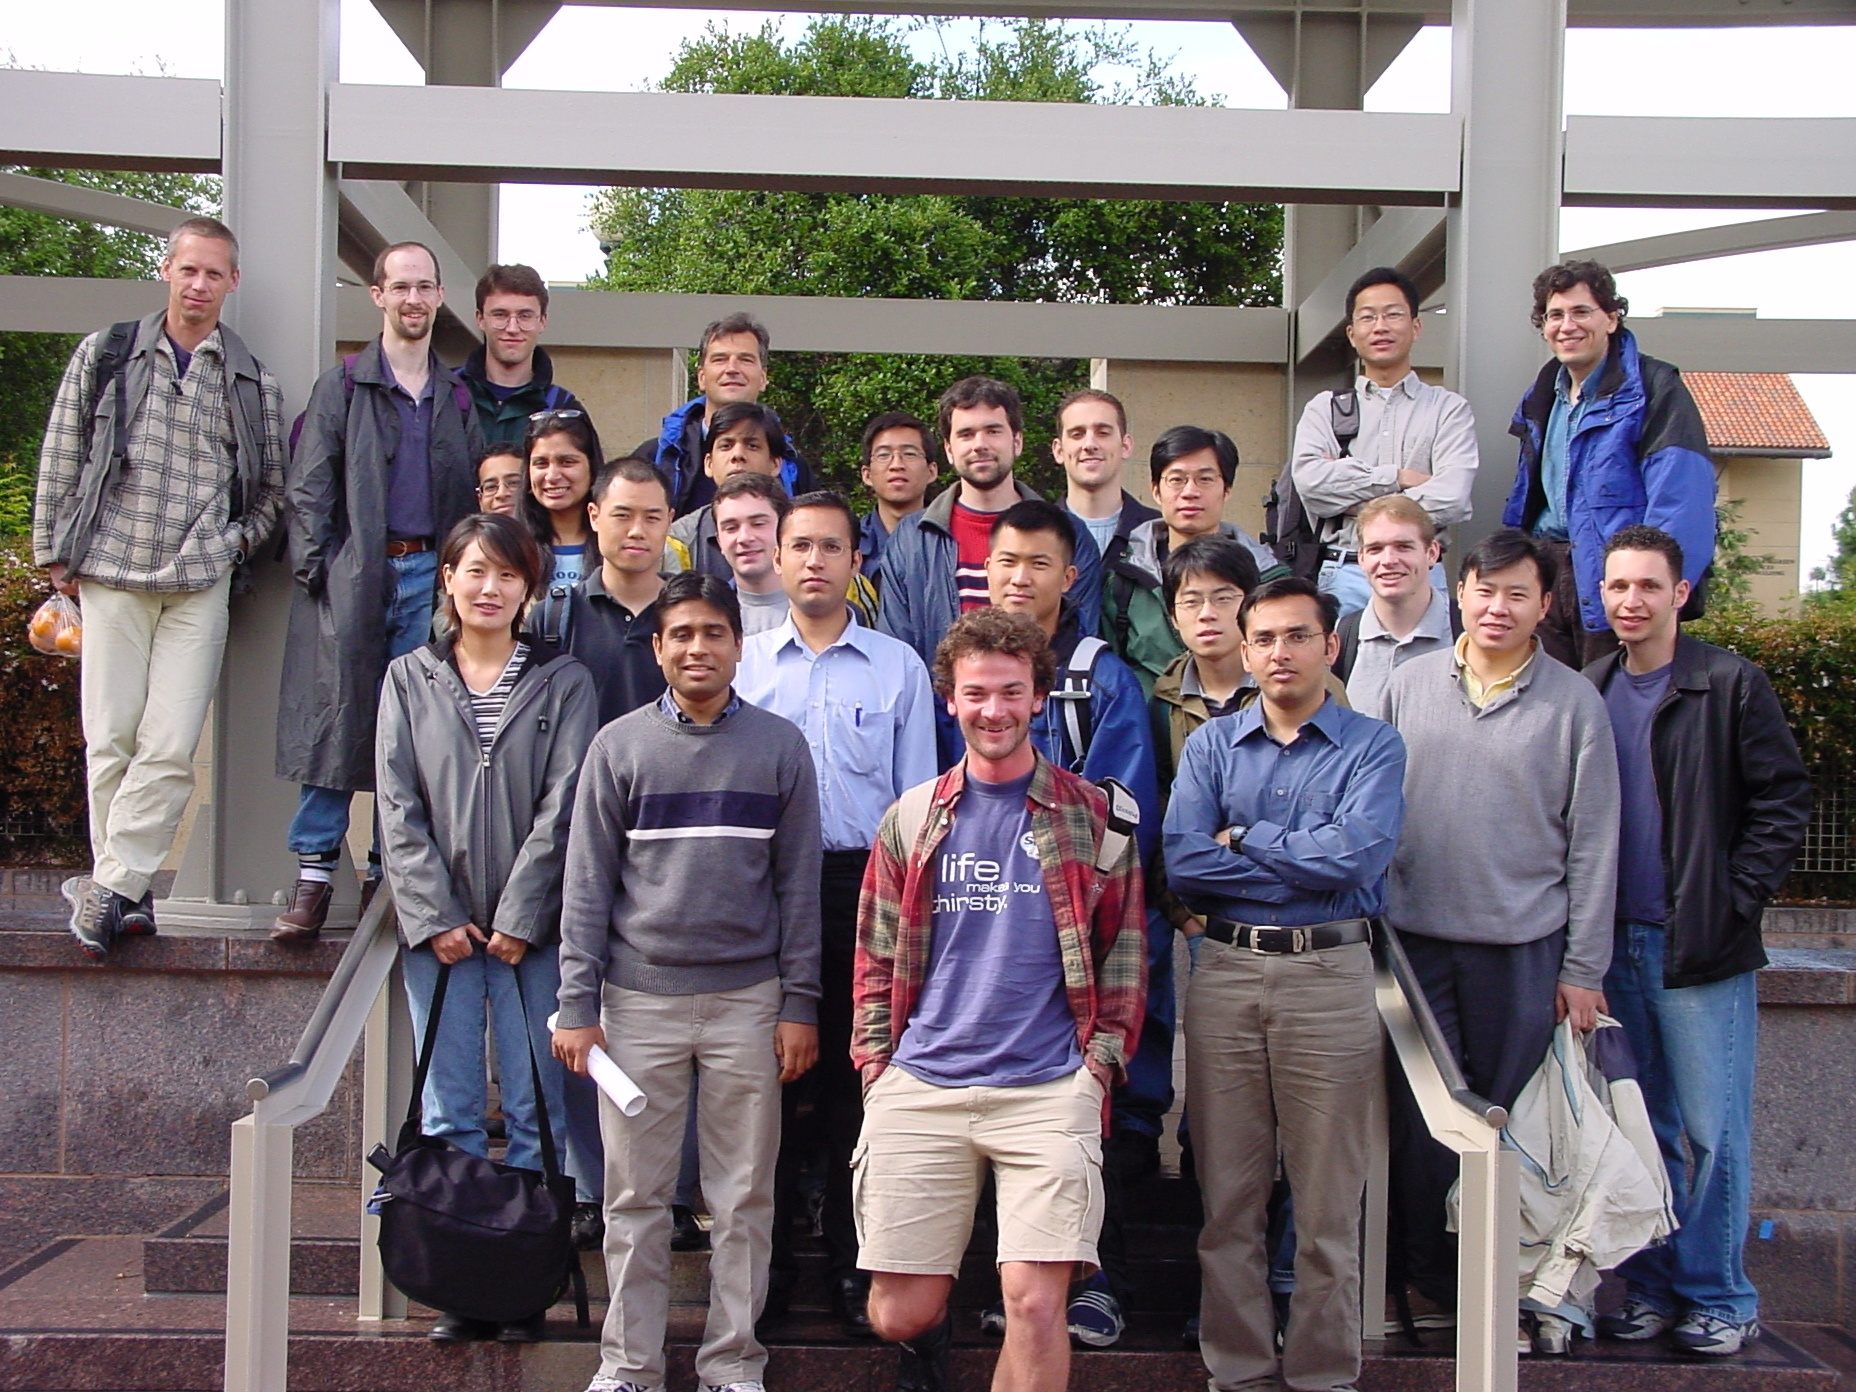
\includegraphics[width=\textwidth]{../output/training_3.jpg}
        \caption{Original}
    \end{subfigure}
    \begin{subfigure}[t]{0.35\textwidth}
        \centering
        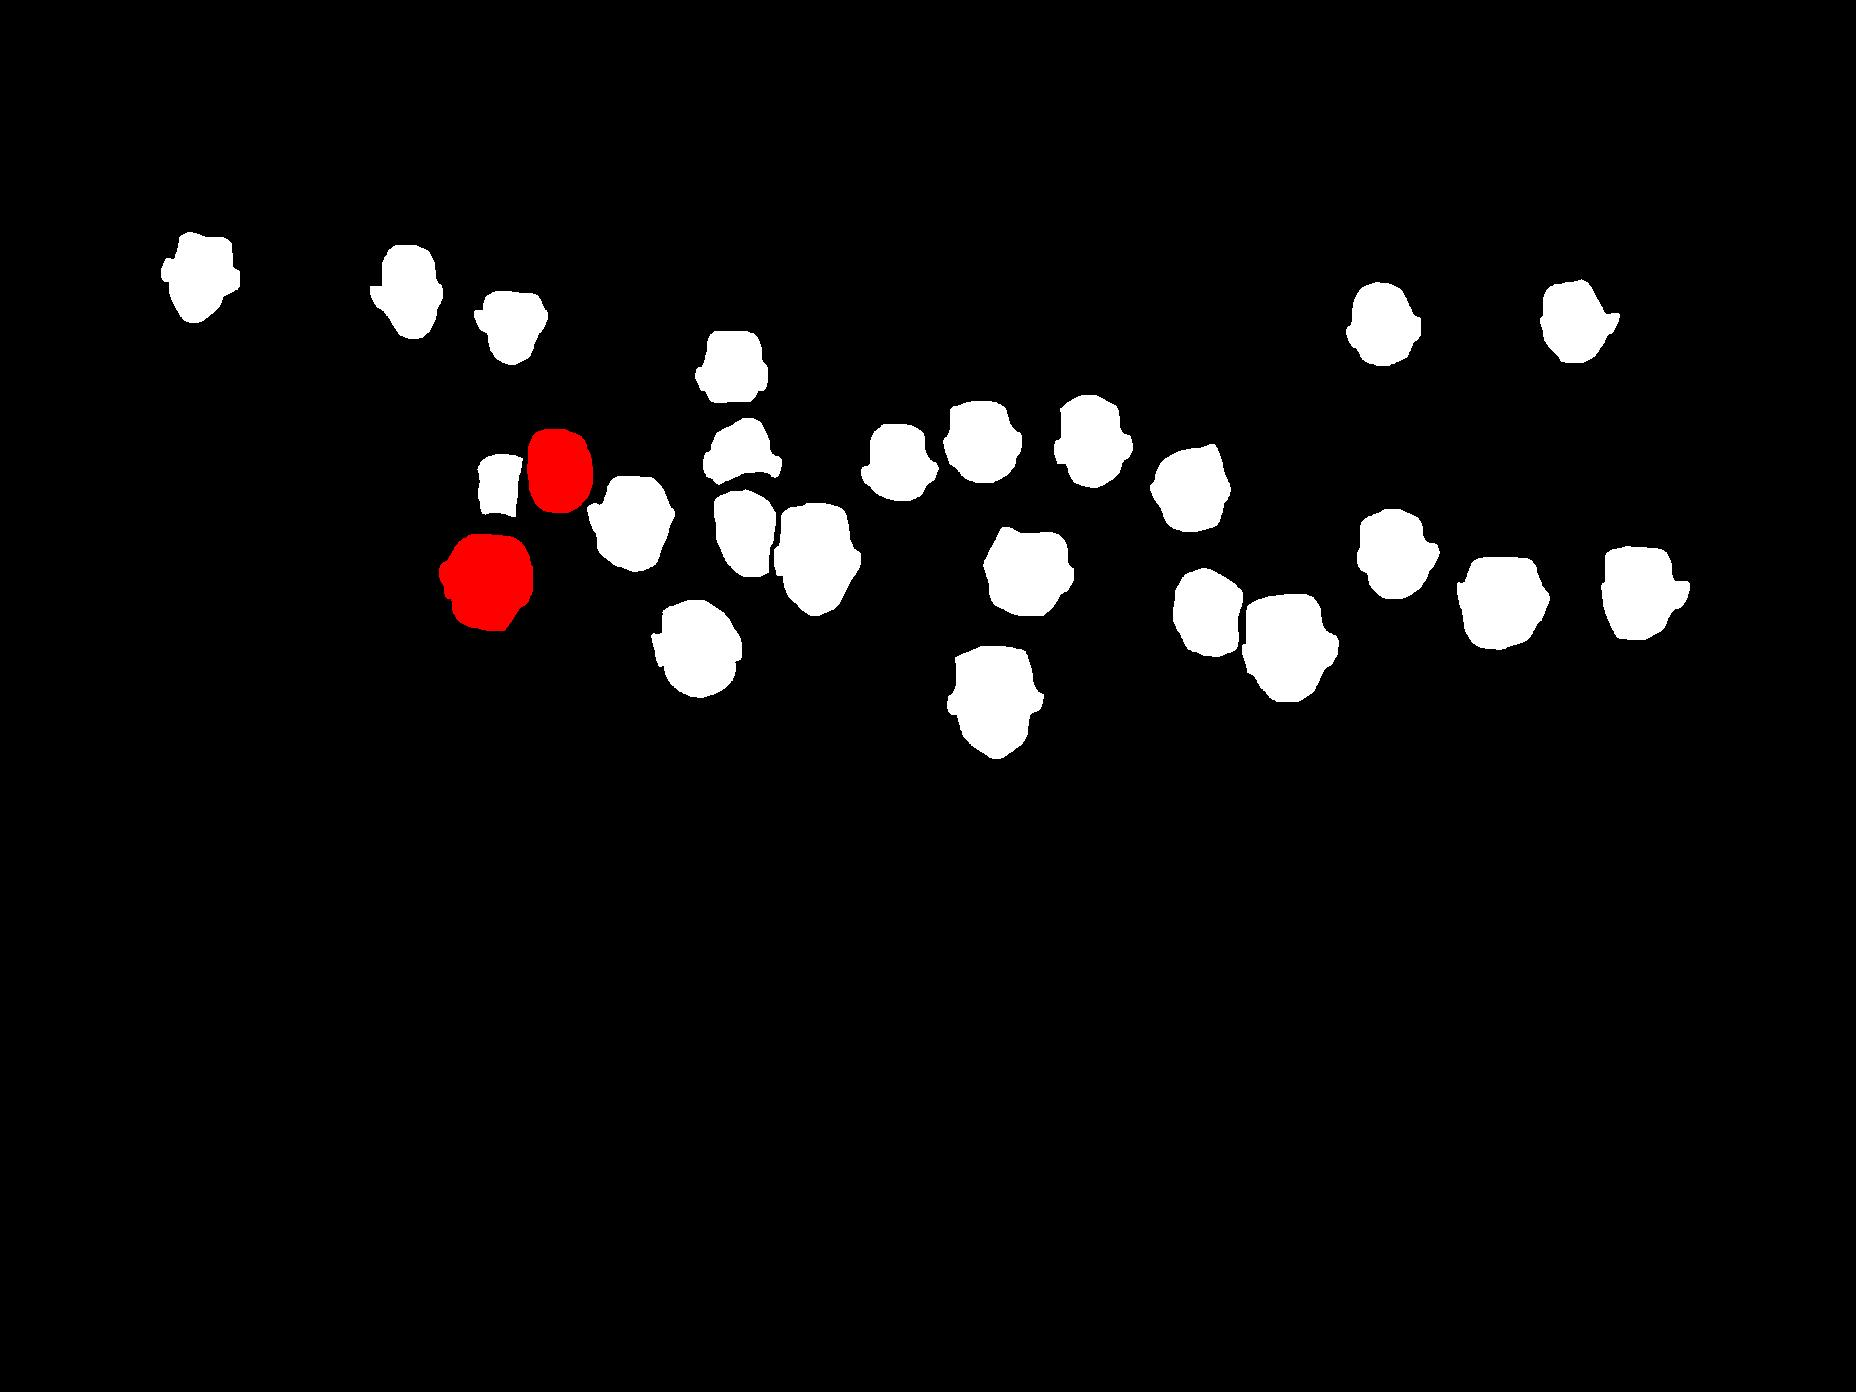
\includegraphics[width=\textwidth]{../output/ref3.jpg}
        \caption{Reference}
    \end{subfigure}
    \par\smallskip
    \begin{subfigure}[t]{0.35\textwidth}
        \centering
        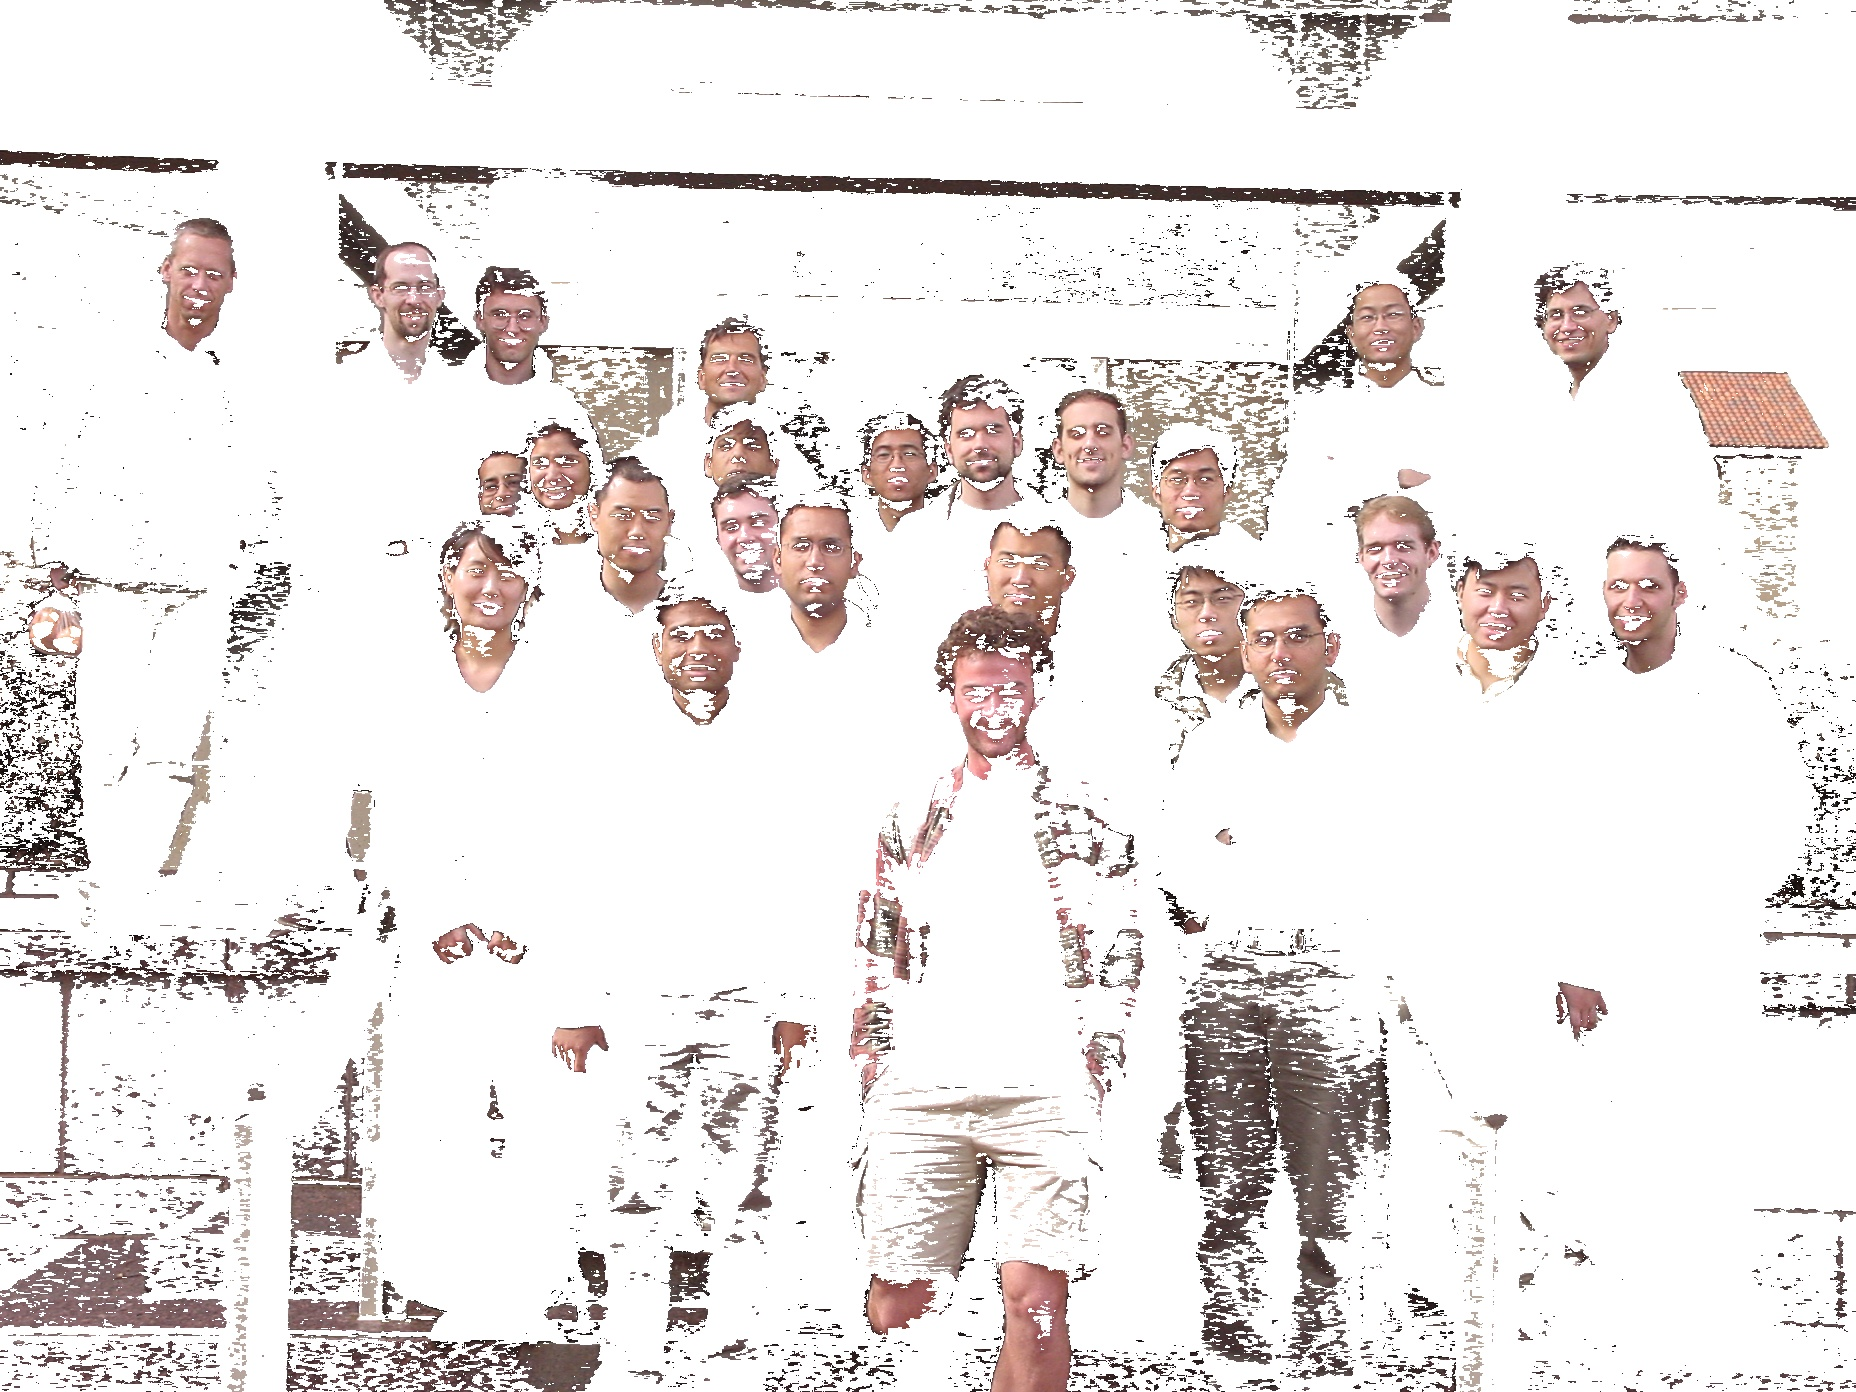
\includegraphics[width=\textwidth]{../output/training_3_a_result.jpg}
        \caption{Result A}
    \end{subfigure}
    \begin{subfigure}[t]{0.35\textwidth}
        \centering
        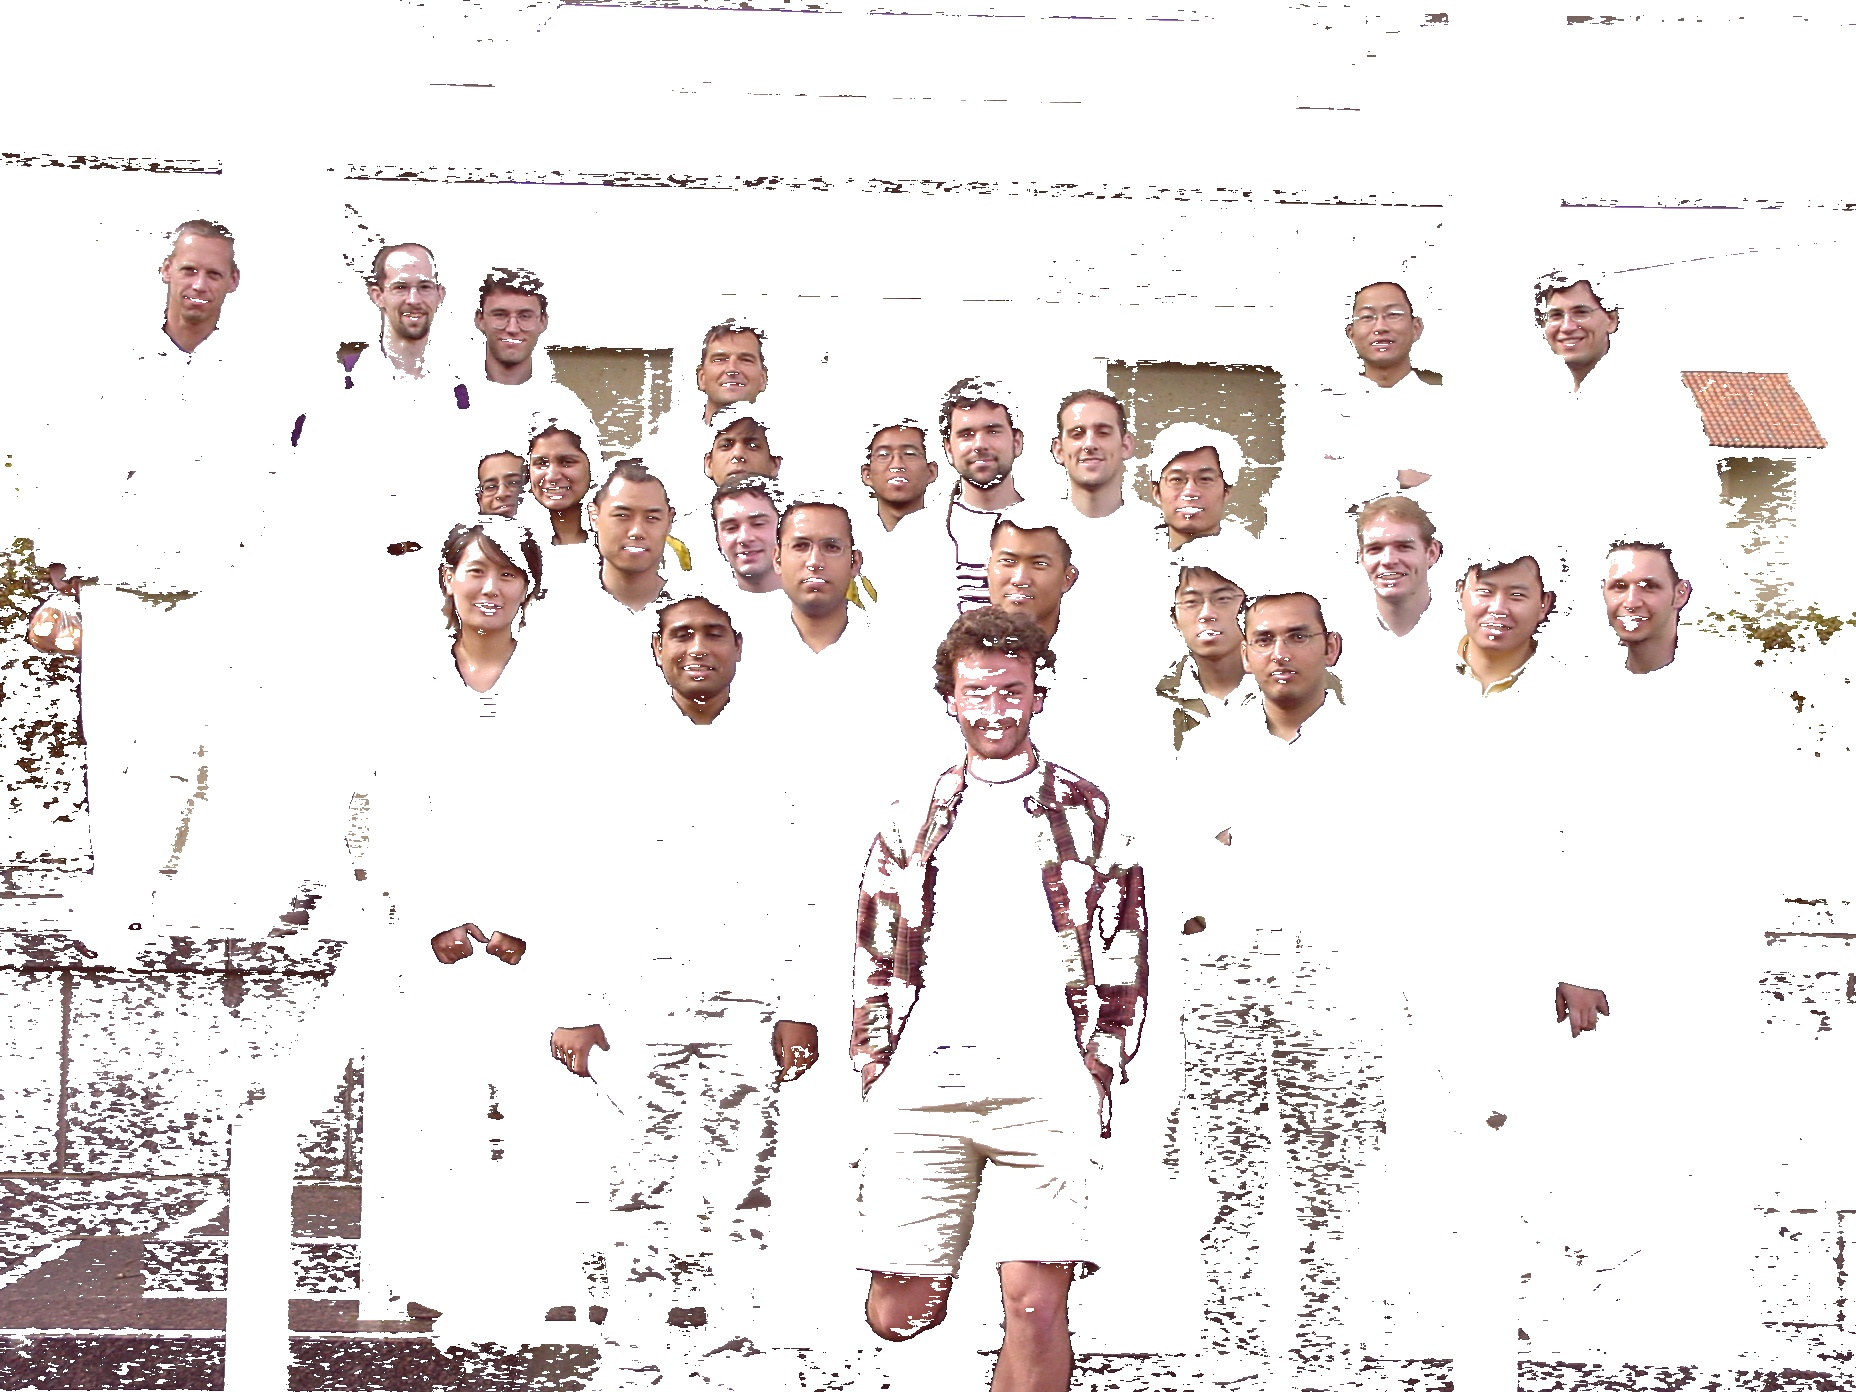
\includegraphics[width=\textwidth]{../output/training_3_b_result.jpg}
        \caption{Result B}
    \end{subfigure}
    \caption{Training 3 Classification Results}
    \label{fig:training3-results}
\end{figure}

\begin{figure}[H]
    \centering
    \begin{subfigure}[t]{0.35\textwidth}
        \centering
        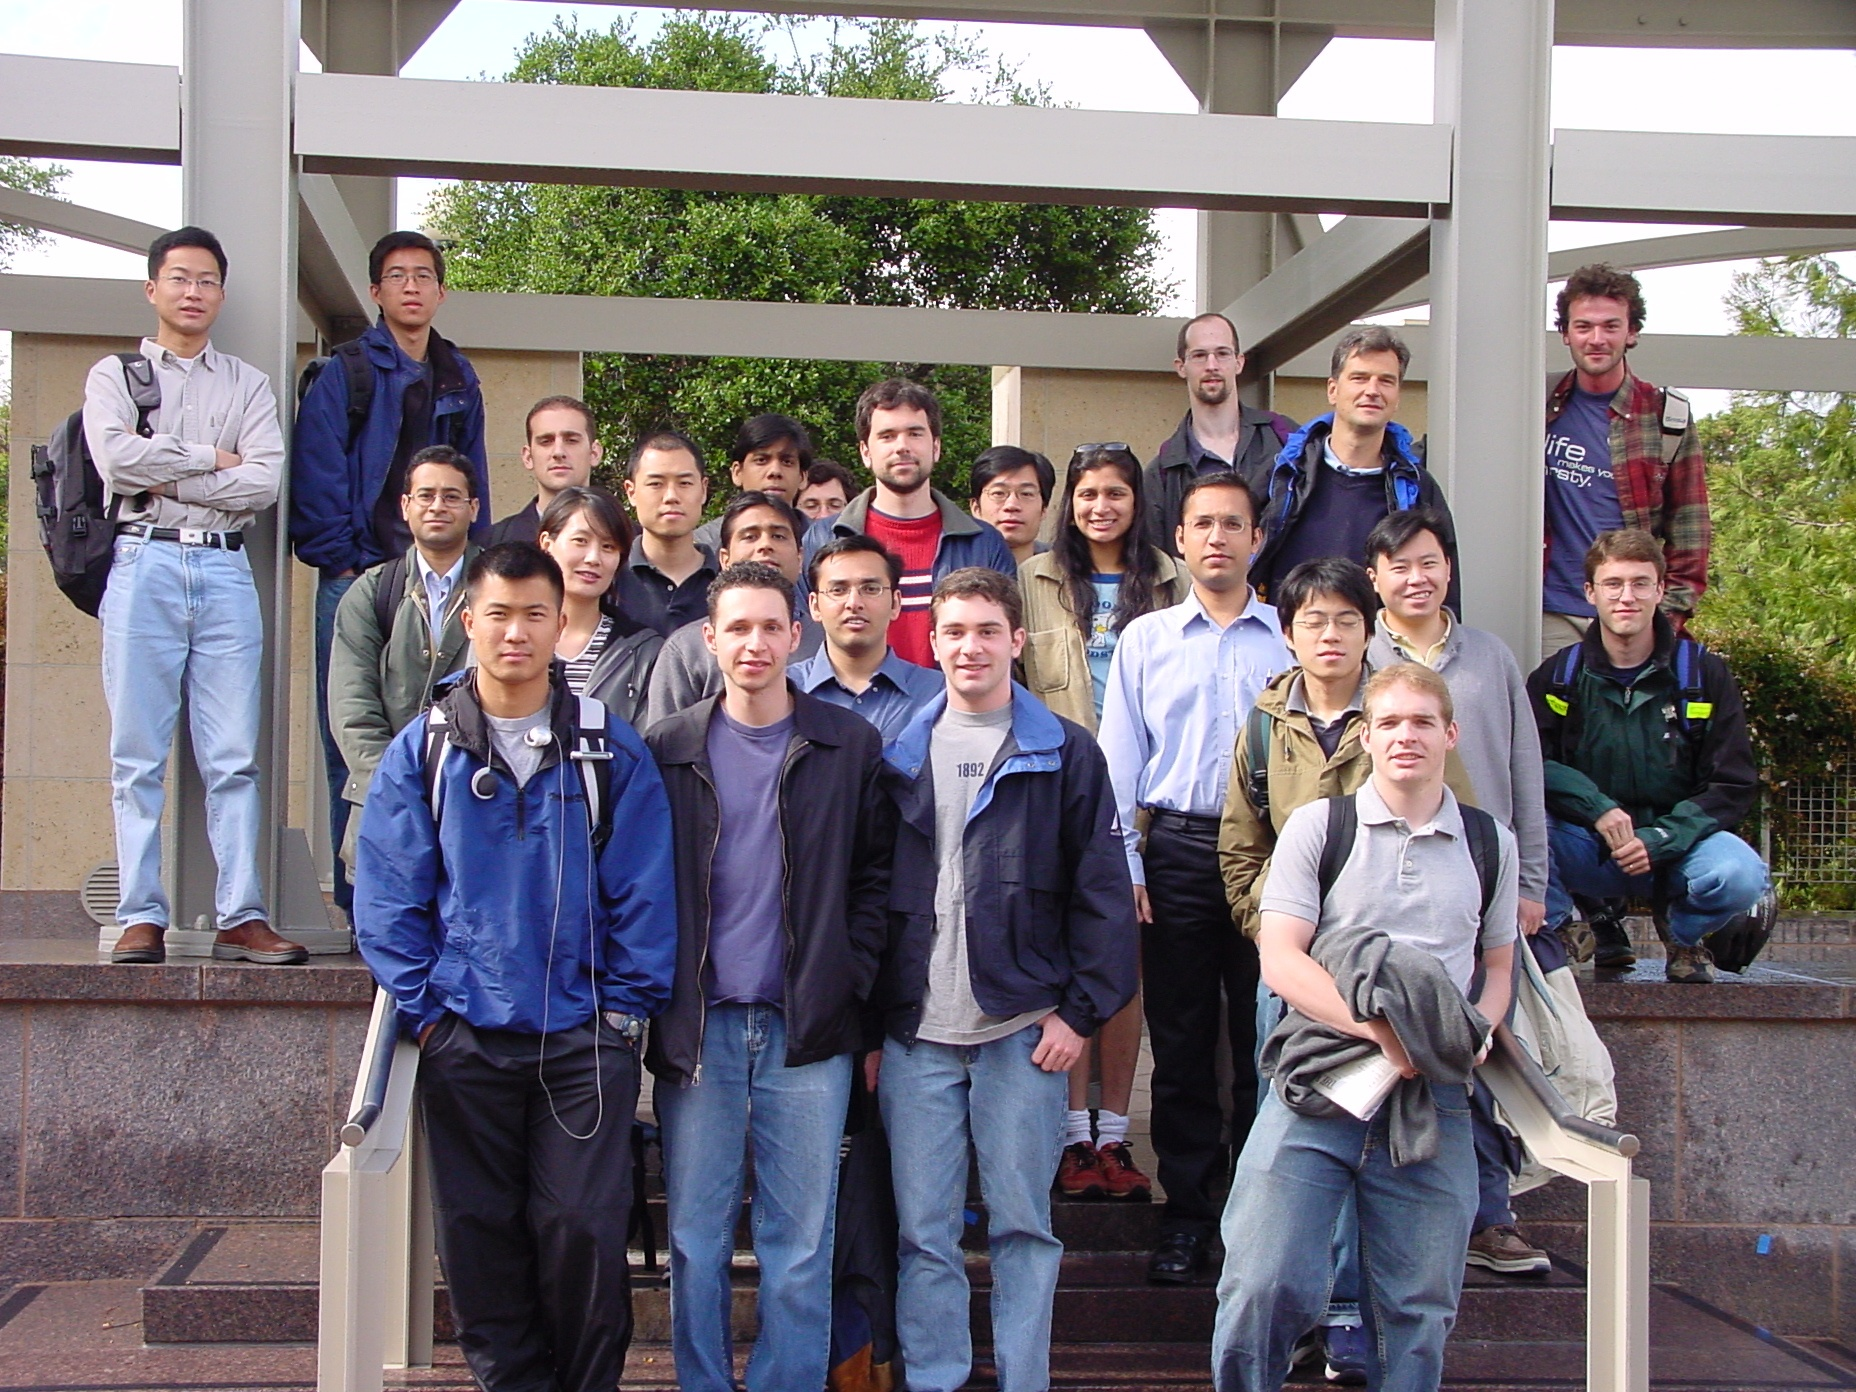
\includegraphics[width=\textwidth]{../output/training_6.jpg}
        \caption{Original}
    \end{subfigure}
    \begin{subfigure}[t]{0.35\textwidth}
        \centering
        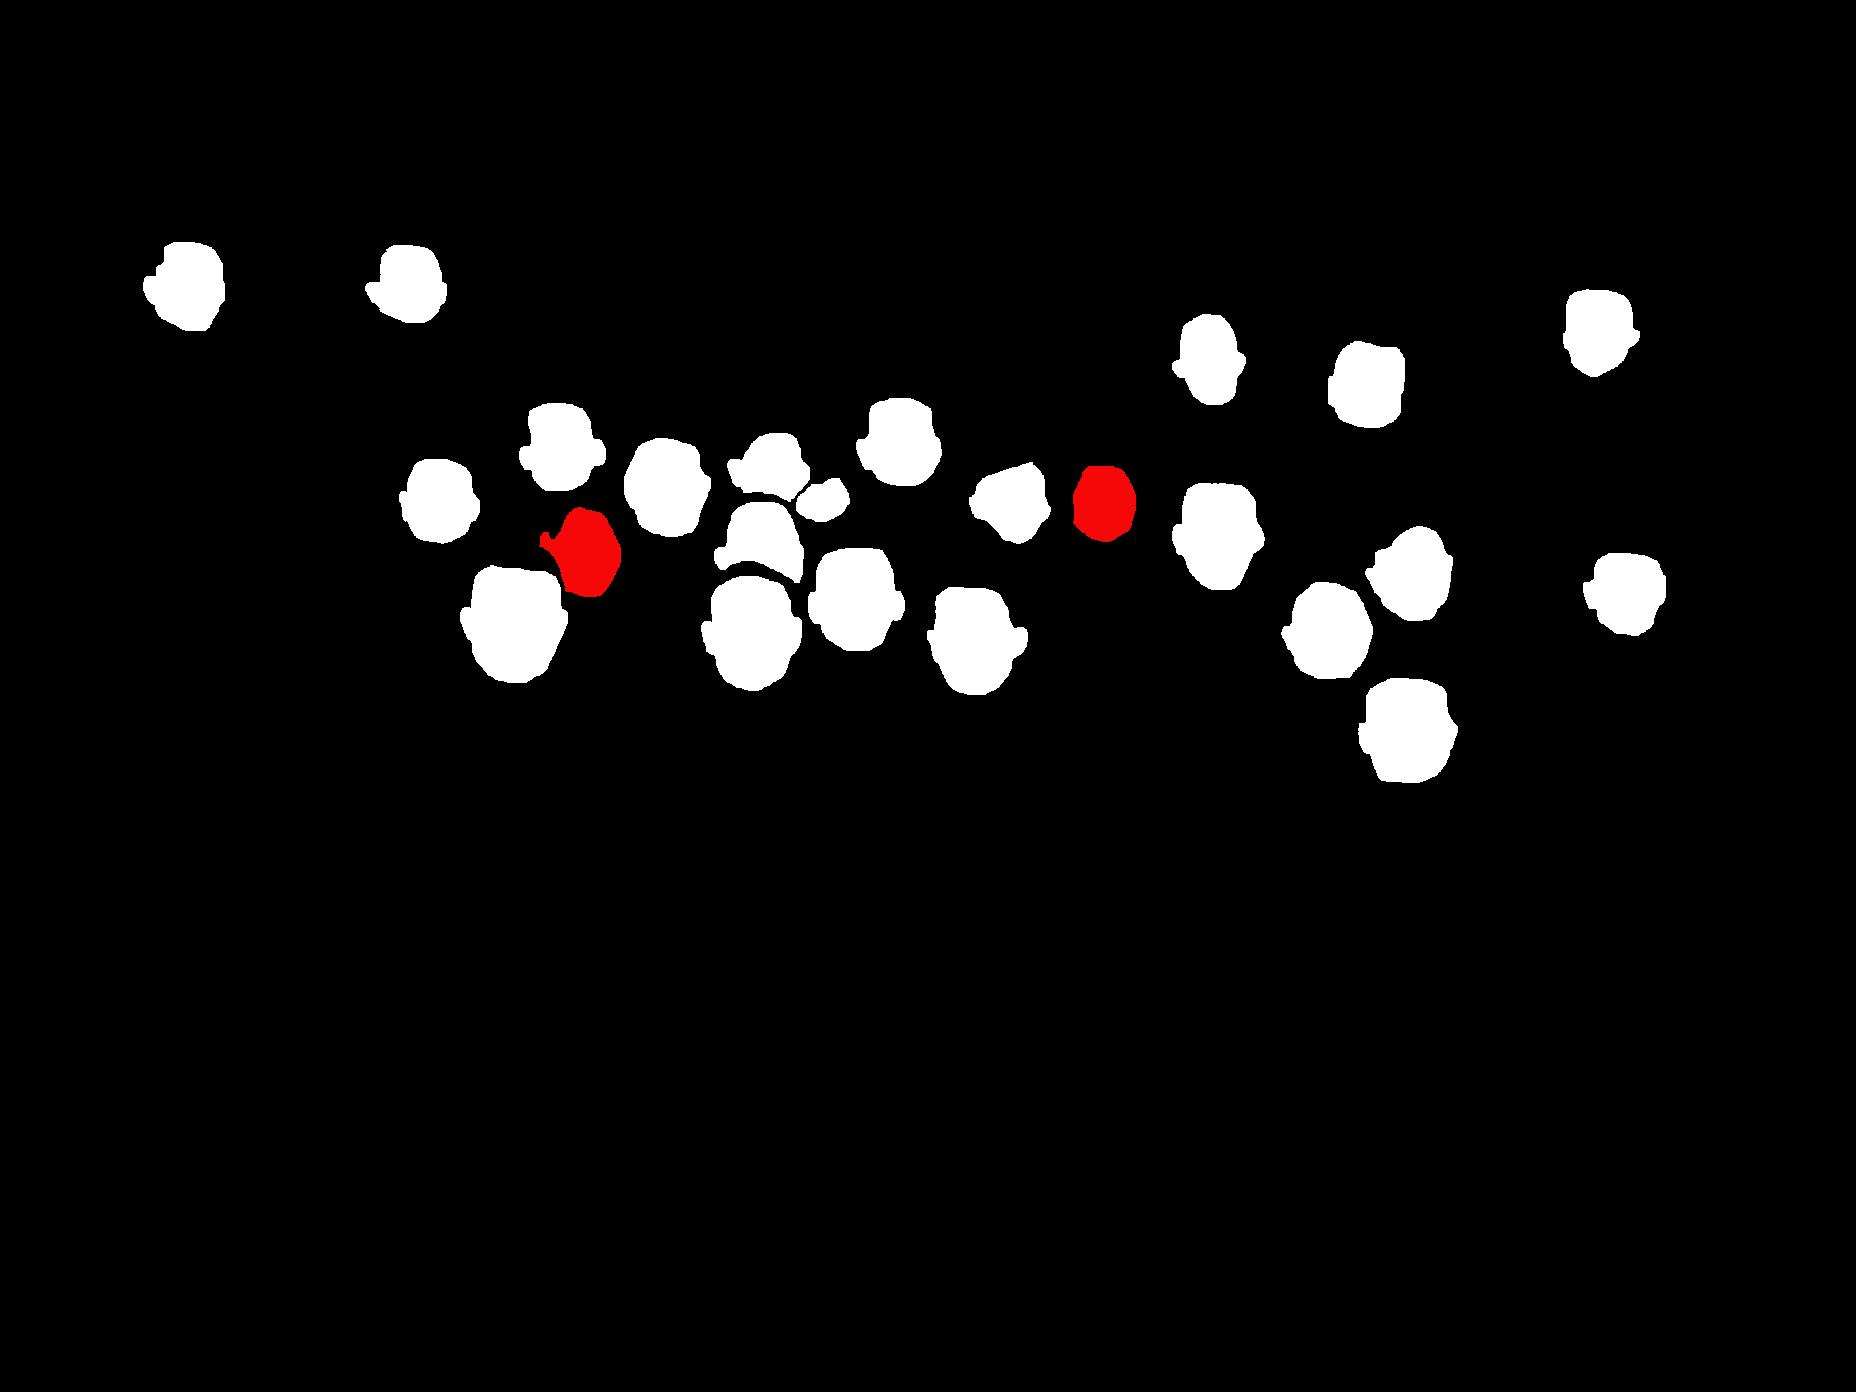
\includegraphics[width=\textwidth]{../output/ref6.jpg}
        \caption{Reference}
    \end{subfigure}
    \par\smallskip
    \begin{subfigure}[t]{0.35\textwidth}
        \centering
        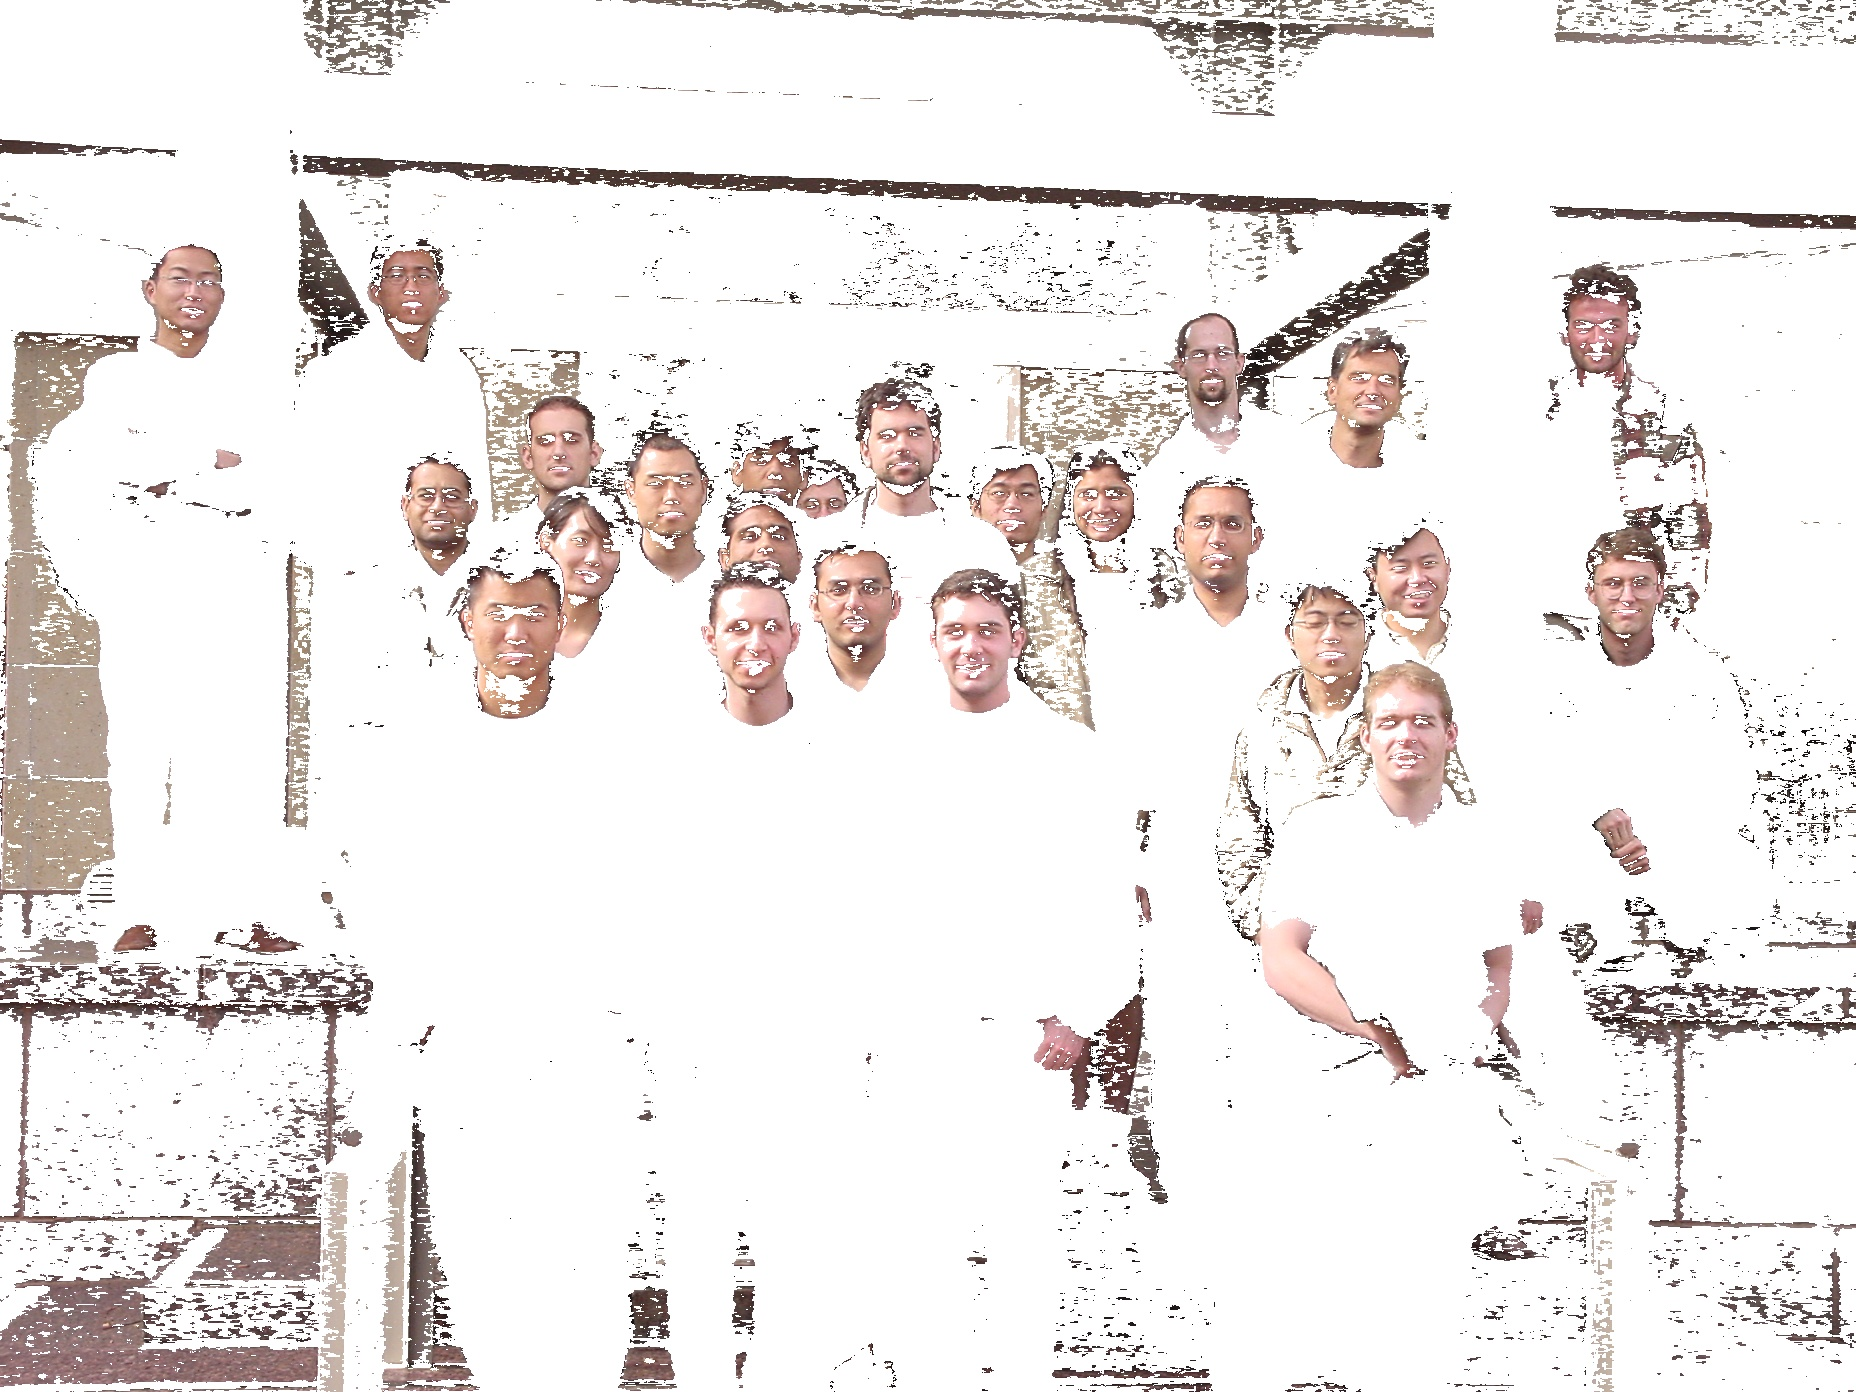
\includegraphics[width=\textwidth]{../output/training_6_a_result.jpg}
        \caption{Result A}
    \end{subfigure}
    \begin{subfigure}[t]{0.35\textwidth}
        \centering
        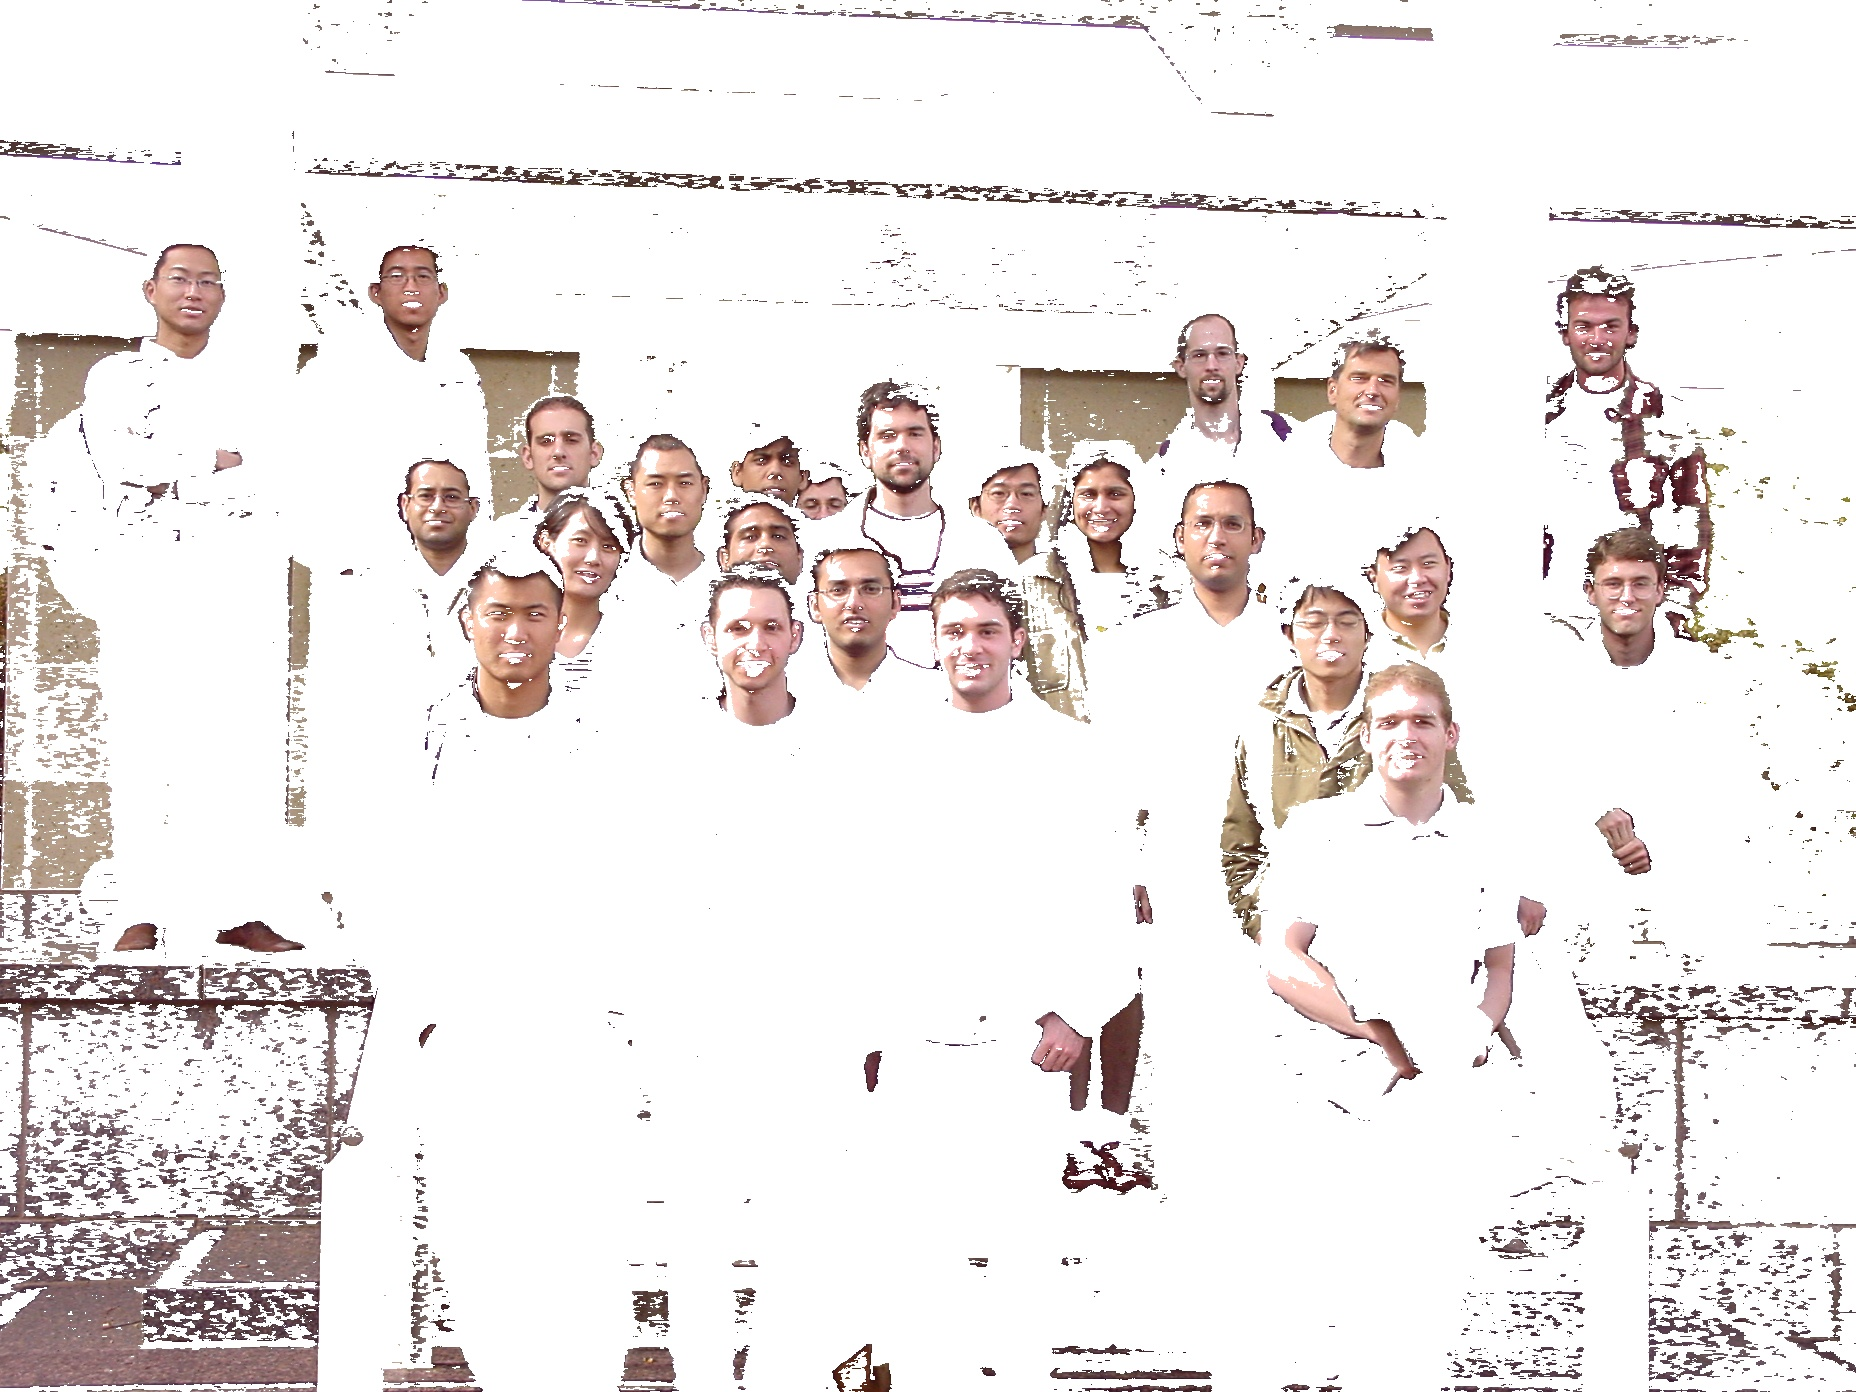
\includegraphics[width=\textwidth]{../output/training_6_b_result.jpg}
        \caption{Result B}
    \end{subfigure}
    \caption{Training 6 Classification Results}
    \label{fig:training6-results}
\end{figure}

As shown in the figures, the YCbCr space classifier seemed to perform better than the normalized RGB space classifier. 
Its output contained less False Positives, agreeing with the data seen in Figure 2. 

Figure 5, below, shows a comparison of the ROC curve for part a, vs the ROC curve for part b. 

\begin{figure}[H]
    \centering
    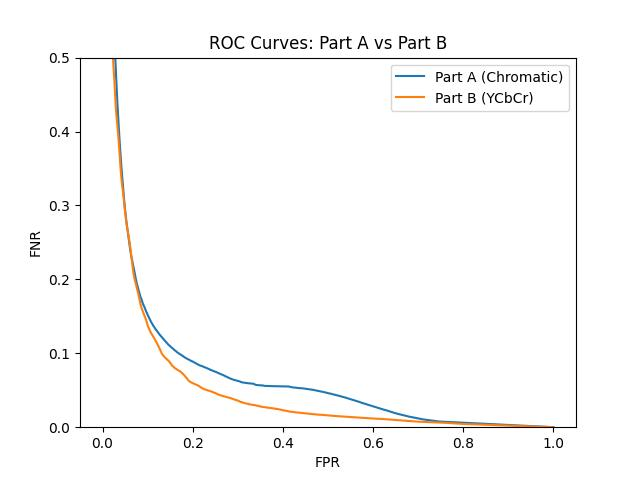
\includegraphics[width=0.48\textwidth]{../output/a_b_roc_curves.jpg}
    \caption{ROC Curves Comparison}
    \label{fig:roc-combined}
\end{figure}

As seen in Figure 5, the area under the ROC curve is smaller for Part B than for Part A. This shows that the YCbCr space likely
performs better overall at separating the luminance from the color information in an image, making it more suitable for 
segmentation purposes in this experiment. 

\end{document}
